\documentclass[a4paper, 12pt]{article}

% Добавляем новые пакеты
\usepackage[english, russian]{babel}    % Пакет для поддержки русского языка
\usepackage[T1, T2A]{fontenc}           % Загружаем пакет с поддержкой кирилицы
\usepackage[utf8]{inputenc}             % Загружаем пакет с поддержкой кодировки файла и символов
\usepackage{ragged2e}                   % Загружаем пакет для выравнивания текста
\usepackage{graphicx}                   % Загружаем пакет для добавления различной графики (pdf, jpg, png)
\usepackage{import}                     % Загружаем пакет для продвинутого импорта, в частности изображений pdf_tex из графического редактора inkscape (\import{<path to file>}{<filename>.pdf_tex})
\usepackage{subcaption}                 % Пакет для поддержки сетки из фигур, например в две колонки или матрицей
\usepackage{float}                      % Пакет для улучшенного размещения изображенией (ниже используется опция H в команде \begin{figure}[H])
\usepackage{geometry}                   % Пакет для управления отступами на странице (см. далее вызываем \geometry)
\usepackage{amsmath}                    % Добавляем крутую поддержку математики, в частности /align
\usepackage{amsfonts}                   % Пкет с мтематическими шрифтами вроде \mathbb и др.
\usepackage{tabu}                       % Пакет с прокаченными таблицами
\usepackage{booktabs}                   % Крутые вертикальные разделители
\usepackage[dvipsnames]{xcolor}         % Рассширенная поддержка цветов
\usepackage[colorlinks]{hyperref}
\usepackage{indentfirst}                % Пакет, чтобы починить красную строку
\usepackage{listings}                   % Поддержка листингов, оформления кода программы
\usepackage{src/vpdtitle}               % Титульный лист (смотри файл vpdtitle.sty)
\usepackage{multirow}
\usepackage{titletoc}
\usepackage{textcomp}
\dottedcontents{section}[2.3em]{}{2.3em}{6pt}
\dottedcontents{subsection}[2.3em]{}{2.3em}{6pt}
\dottedcontents{subsubsection}[2.3em]{}{2.3em}{6pt}

% Устанавливает отступы на странице
\geometry{left=2cm, right=2cm, bottom=2cm, top=2cm}

% Настараиваем красивые цвета для ссылок на формулы, фигуры (изображения) и другие элементы.
\hypersetup{
    linkcolor=blue,
    filecolor=magenta,
    urlcolor=cyan
}

% Настраиваем супер красивые листинги с попомщью пакетов listings и xcolor
\definecolor{codegreen}{rgb}{0,0.6,0}
\definecolor{codegray}{rgb}{0.5,0.5,0.5}
\definecolor{codepurple}{rgb}{0.58,0,0.82}
\definecolor{backcolour}{rgb}{0.95,0.95,0.92}

\lstdefinestyle{codestyle}{
    backgroundcolor=\color{backcolour},
    commentstyle=\color{codegreen},
    keywordstyle=\color{magenta},
    numberstyle=\tiny\color{codegray},
    stringstyle=\color{codepurple},
    basicstyle=\ttfamily\footnotesize,
    breakatwhitespace=false,
    breaklines=true,
    captionpos=b,
    keepspaces=true,
    numbers=left,
    numbersep=5pt,
    showspaces=false,
    showstringspaces=false,
    showtabs=false,
    tabsize=2
}

\lstset{style=codestyle}
\lstset{extendedchars=\true}

%%%%%%%%%%%%%%%%%%%%%%%%%%%%%%%%%%%%%%%%%%%%%%%%
%% Заполнение титульного листа
%%%%%%%%%%%%%%%%%%%%%%%%%%%%%%%%%%%%%%%%%%%%%%%%
\title{
Точностные свойства систем
}

% Тут укажите автора
\author{Иван М. Бакланов}
\affil{465112, ibaklanov@niuitmo.ru}

\author{Владимир В. Ананичев}
\affil{464994, vandmitrievic@mail.ru}
% Впишите данные о том, кто будет проверять работу
\author{Даниил А. Юлдашев}
\affil{468158}

\supervisor{Артем В. Пашенко}

% Краткое описание того, что сделали в работе
\abstract{
Ознакомление с точностными свойствами линейных систем на примере систем с пропорциональным, интегральным и пропорционально-интегральным регуляторами.
}

% Подберите 3-5 ключевых слова, отличающих эту работу от всех остальных
\keywords{
    Simulink, Matlab, Linear systems, Control theory, установившаяся ошибка
}

\date{\today}







%%%%%%%%%%%%%%%%%%%%%%%%%%%%%%%%%%%%%%%%%%%%%%%%
% Начала всего-всего текста. Здесь идет сам документ, все пишется именно сюда
%%%%%%%%%%%%%%%%%%%%%%%%%%%%%%%%%%%%%%%%%%%%%%%%
\begin{document}

\maketitle

\tableofcontents

\newpage


\section{Задание №1. Пропорциональный регулятор}
\subsection{Схема моделирования системы}
Построим схему моделирования исследуемой системы в Simulink:
\begin{figure}[H]
    \centering
    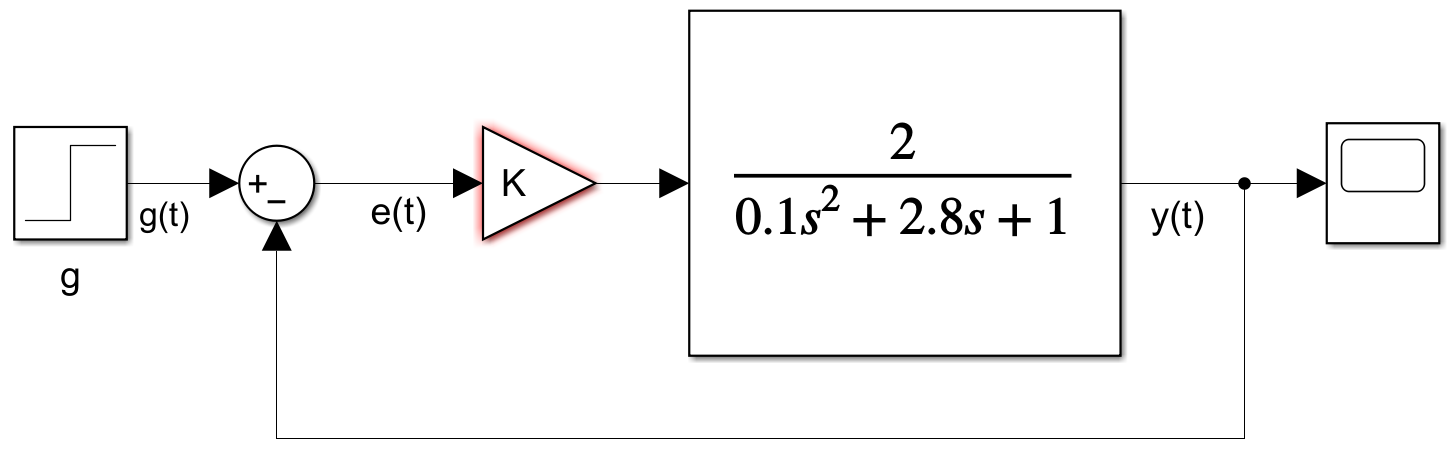
\includegraphics[width=\textwidth]{images/model1.png}
    \caption{Схема моделирования задания 1}
    \label{fig:1}
\end{figure}
При этом, так как начальные условия считаем равными $0$, можем пользоваться блоком simulink transfer fcn для задания передаточной функции управляемого объекта.
\subsection{Аналитический расчет предельного значения установившейся ошибки в стационарном режиме}
Проверим ассимптотическую устойчивость системы. Для этого найдем полную передаточную функцию системы по ошибке как:
\[
    W(s)_{g \rightarrow e} = \frac{1}{1 + H(s)W_{\textit{упр}}(s)} = \frac{1}{\frac{0,1s^2 + 2,8s + 1 + 2K}{0,1s^2 + 2,8s + 1}} = \frac{0,1s^2 + 2,8s + 1}{0,1s^2 + 2,8s + 1 + 2K}
\]
Выразим корни знаменателя:
\[
    \lambda_{1, 2} = \frac{-2,8 \pm \sqrt{2,8 ^ 2 - 4 \cdot 0,1 \cdot (1 + 2K)}}{2 \cdot 0,1}
\]
Видим, что вещественные части обоих корней отрицательны при любом $K > 0$, следовательно, в условиях нашей задачи система ассимптотически устойчива.
\newline
Так как входное воздействие постоянно, можем выразить статическую ошибку как:
\[
    \varepsilon = \frac{1}{1 + K_0}g_0
\]
Где $K_0$ - статический коэффициент передачи, равен:
\[
    K_0 = \frac{b_0}{a_0} = \frac{2K}{1}
\]
$g_0$ - постоянное входное воздействие:
\[
    g(t) = g_0 = A
\]
Таким образом,
\[
    \varepsilon = \frac{A}{1 + 2K} = \frac{3}{1 + 2K}
\]
$K$ равняется $1$, $5$ или $10$ в зависимости от номера эксперимента.
\newpage
\subsection{Сравнительные графики для стационарного режима}
Построим графики $y(t)$ при различных коэффициентах пропорционального регулятора. Также для наглядности построим на этих же осях соответствующие установившиеся значения ($y_{\textit{уст}i} = g0 - \varepsilon_i$) и входное воздействие, соответствующее целевому значению.
\begin{figure}[H]
    \centering
    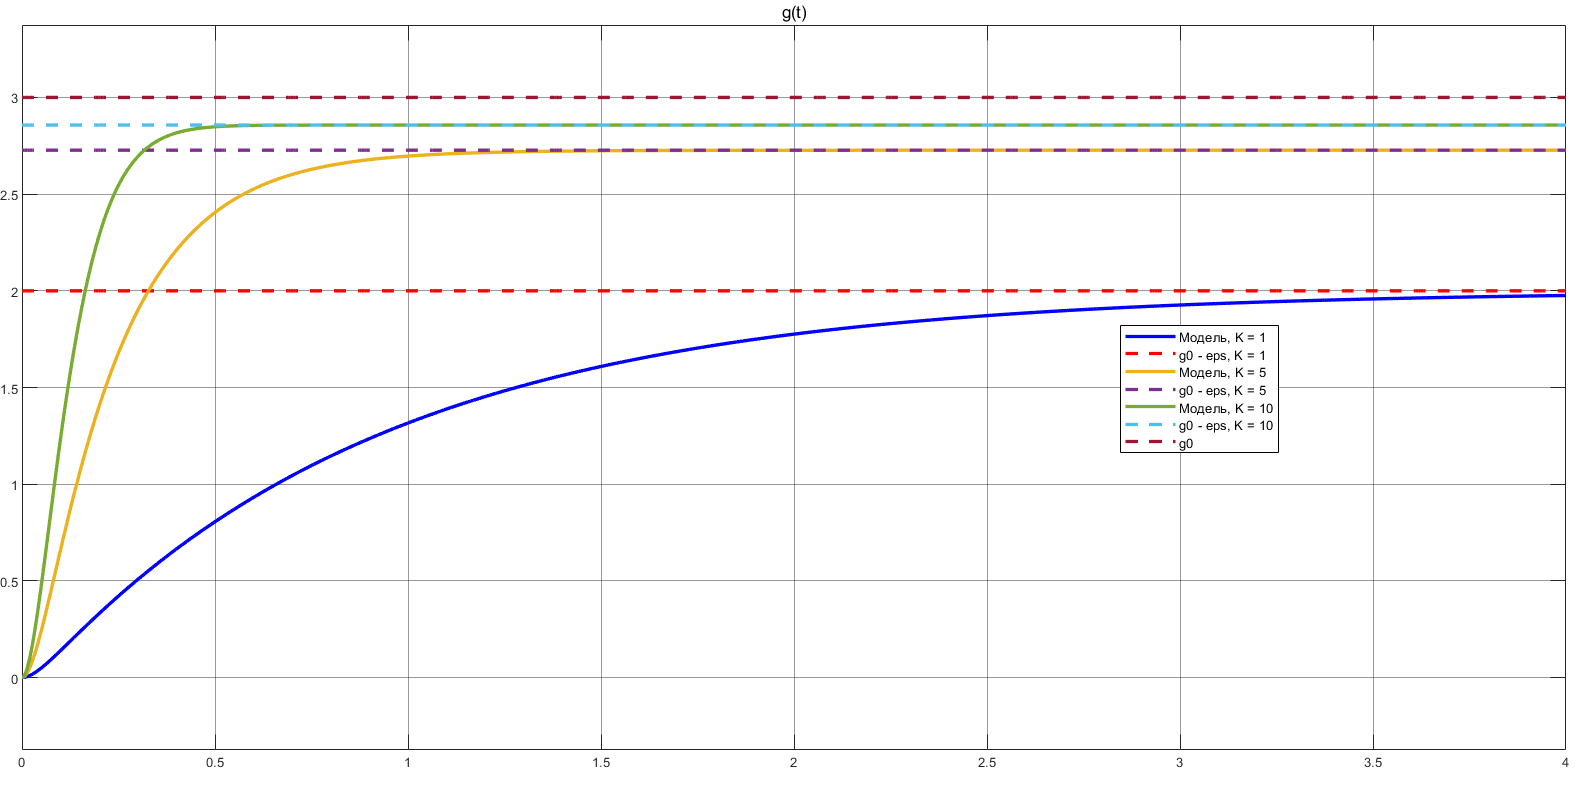
\includegraphics[width=\textwidth]{images/t1g1.png}
    \caption{Сравнительные графики $y(t)$ для задания 1, стационарного режима}
    \label{fig:2}
\end{figure}
Затем построим графики $e(t)$, для наглядности изобразим в тех же осях установившуюся ошибку $\varepsilon$:
\begin{figure}[H]
    \centering
    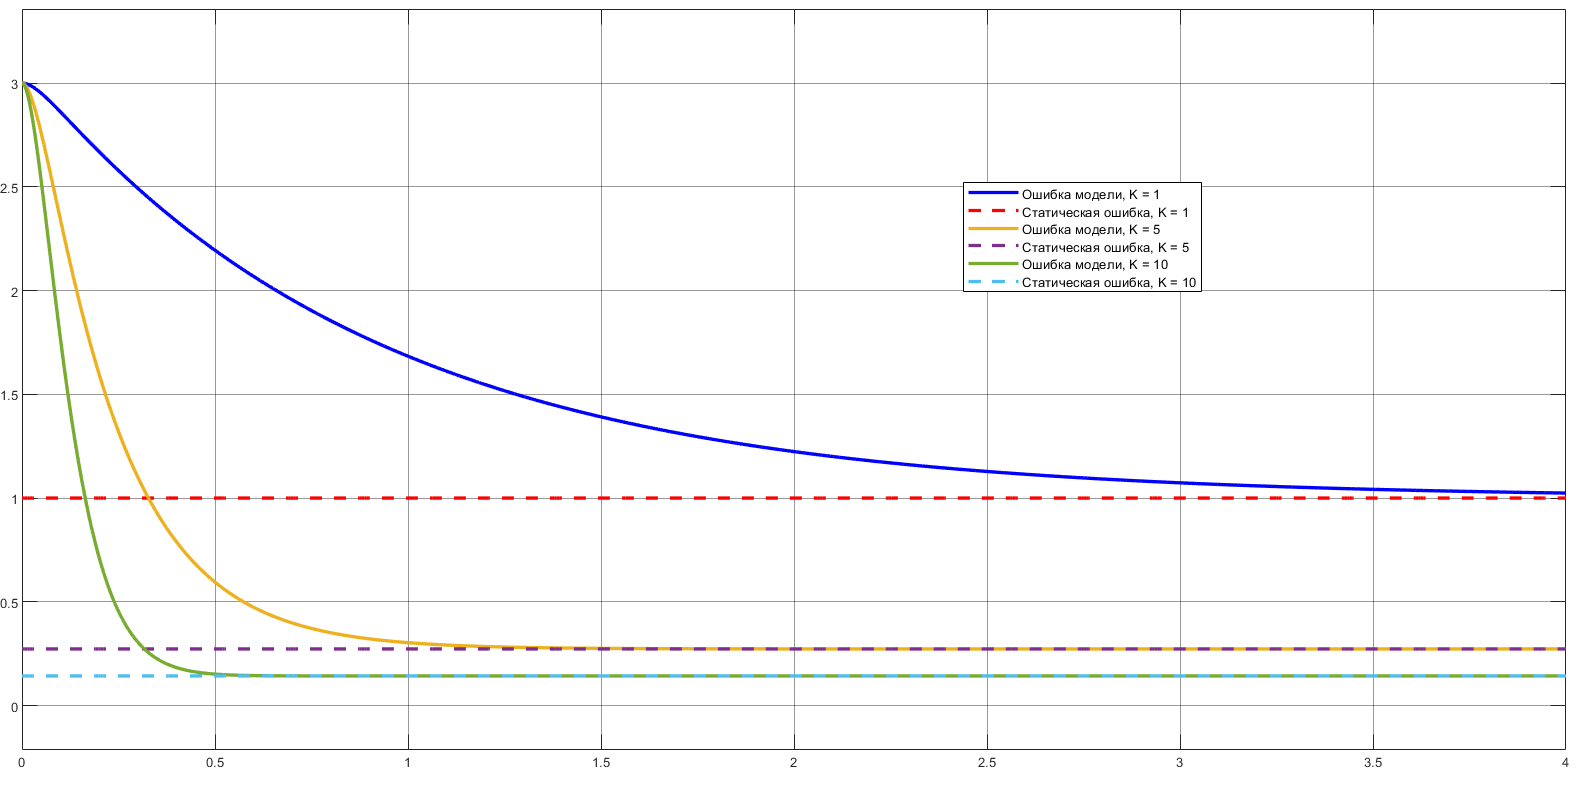
\includegraphics[width=\textwidth]{images/t1g2.png}
    \caption{Сравнительные графики $e(t)$ для задания 1, стационарного режима}
    \label{fig:2}
\end{figure}
\newpage
\subsection{Сравнительные графики для движения с постоянной скоростью}
Теперь зададим входное воздействие как $Vt = 2,5t$ и построим аналогичные сравнительные графики $y(t)$ и $e(t)$:
\begin{figure}[H]
    \centering
    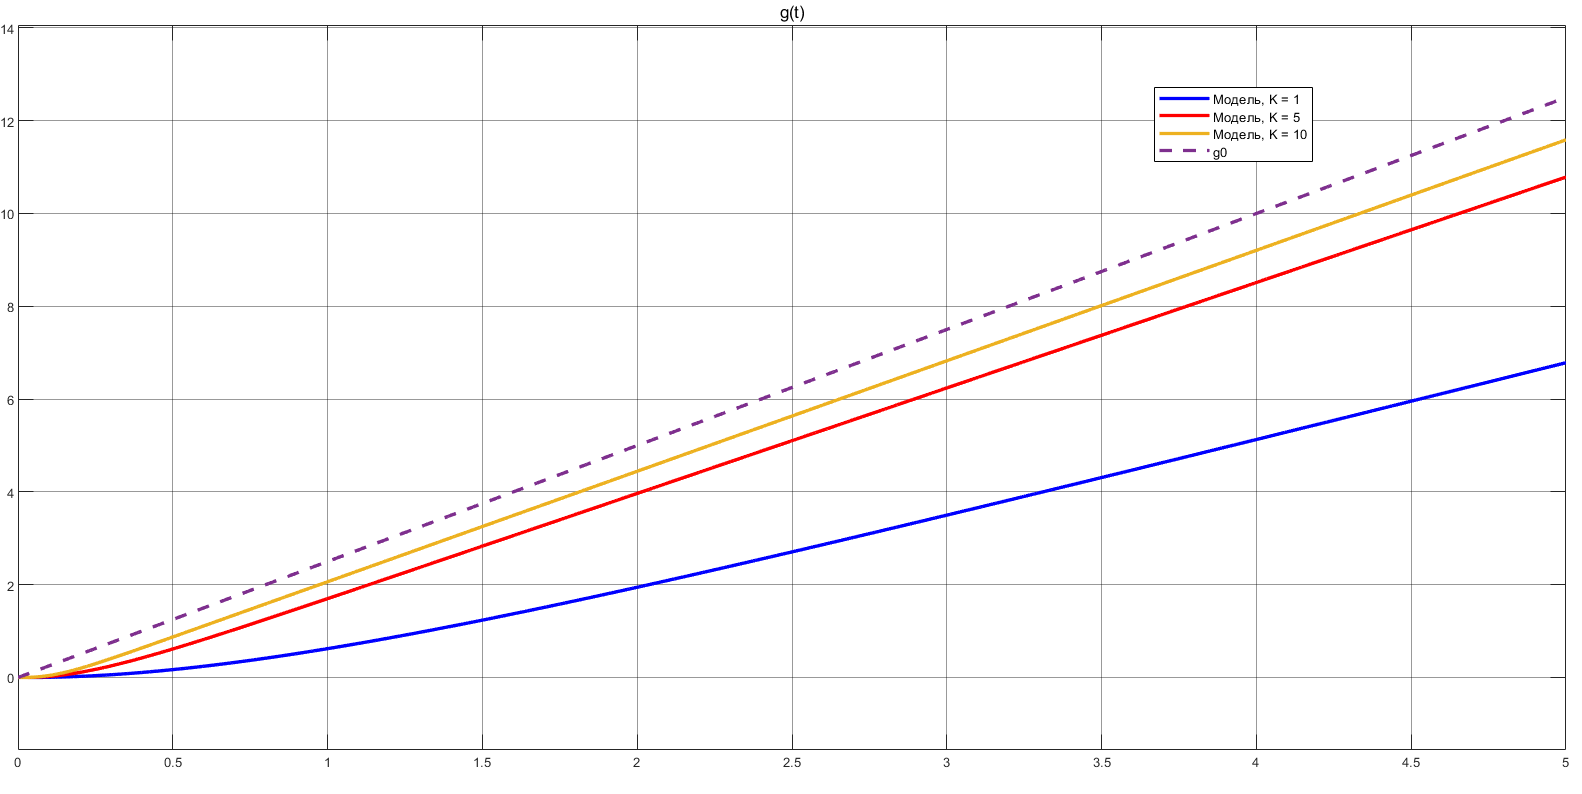
\includegraphics[width=\textwidth]{images/t1g3.png}
    \caption{Сравнительные графики $y(t)$ для задания 1, постоянной скорости}
    \label{fig:2}
\end{figure}
\begin{figure}[H]
    \centering
    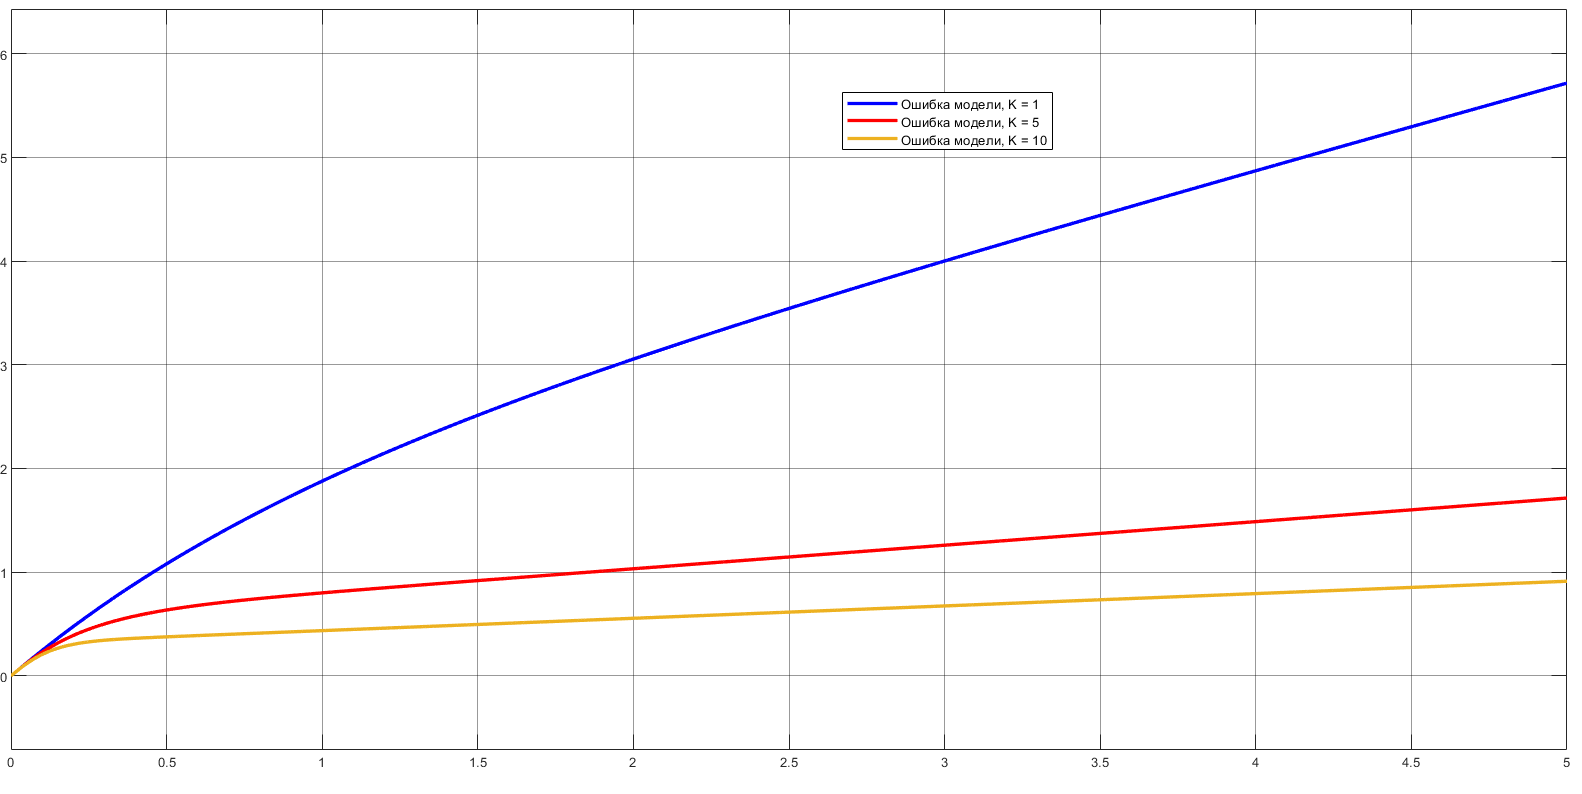
\includegraphics[width=\textwidth]{images/t1g4.png}
    \caption{Сравнительные графики $e(t)$ для задания 1, постоянной скорости}
    \label{fig:2}
\end{figure}
\newpage
\subsection{Выводы по заданию 1}
В результате моделирования линейной системы с пропорциональным регулятором в стационарном режиме было получено соответствие вычисленной теоретически статической ошибки и результатов моделирования. Также из результатов моделирования можно сделать вывод что при увеличении коэффициента пропорционального регулятора установившаяся ошибка и время переходного процесса уменьшаются.
\newline
При моделировании же этой системы в режиме движения с постоянной скоростью было получено, что ошибка неограничено возрастает с течением времени (что соответствует нулевому порядку астатизма системы). При этом увеличение коэффициента пропорционального регулятора снижает скорость роста ошибки.
\newpage
\section{Интегральный регулятор}
\subsection{Схема моделирования системы}
Построим схему моделирования исследуемой системы в Simulink, заменив в прошлой схеме функцию регулятора:
\begin{figure}[H]
    \centering
    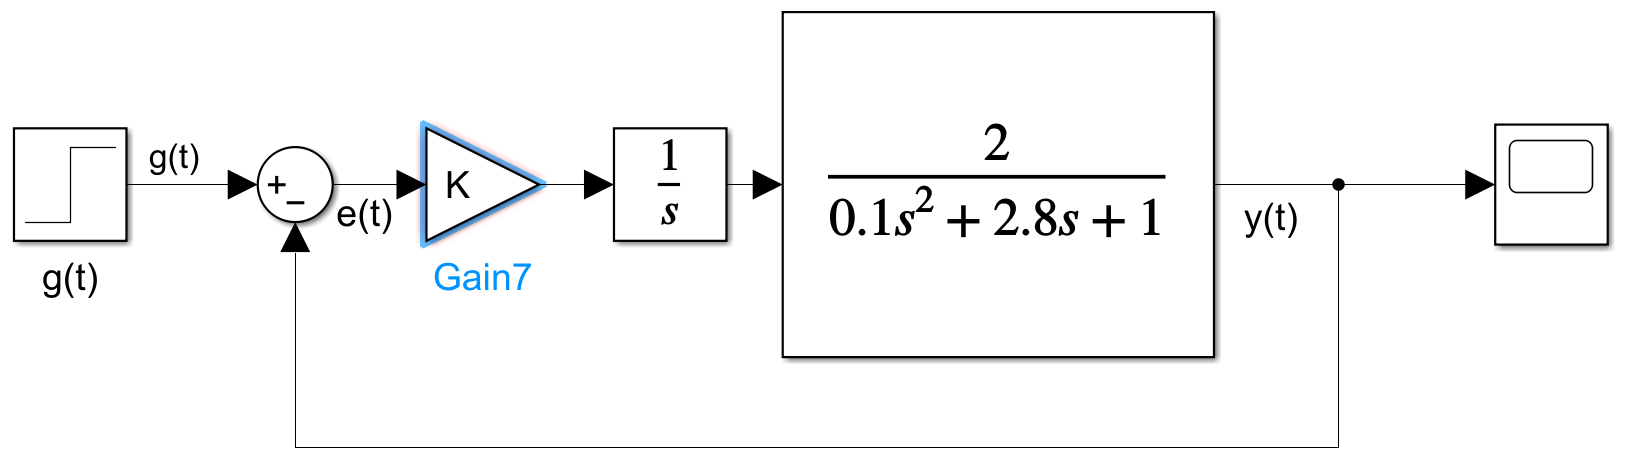
\includegraphics[width=\textwidth]{images/model2.png}
    \caption{Схема моделирования задания 2}
    \label{fig:1}
\end{figure}
\subsection{Аналитический расчет предельного значения установившейся ошибки}
Проверим ассимптотическую устойчивость системы. Для этого найдем полную передаточную функцию системы по ошибке как:
\[
    W(s)_{g \rightarrow e} = \frac{1}{1 + H(s)W_{\textit{упр}}(s)} = \frac{1}{\frac{0,1s^3 + 2,8s^2 + s + 2K}{0,1s^3 + 2,8s^2 + s}} = \frac{0,1s^3 + 2,8s^2 + s}{0,1s^3 + 2,8s^2 + s + 2K}
\]
Составим матрицу Гурвица:
\[
    H = \begin{pmatrix}
    2,8 & 2K & 0 \\
    0,1 & 1 & 0 \\
    0 & 2,8 & 2K
\end{pmatrix}
\]
Найдем определители ее угловых матриц:
\[
    \Delta_1 = 2,8
\]
\[
    \Delta_2 = 2,8 - 0,2K
\]
\[
    \Delta_3 = 5,6K - 0,4K^2
\]
При $K < 14$ все определители положительны, следовательно, в условиях нашей задачи система ассимптотически устойчива.
\newline
Порядок астатизма системы равен 1, следовательно в стационарном режиме:
\[
    \varepsilon = 0
\]
В режиме движения с постоянной скоростью статическая ошибка равна:
\[
    \varepsilon = \frac{V}{K_1} = \frac{2,5}{\frac{2K}{1}} = \frac{2,5}{2K}
\]
Теперь можем построить для системы с интегральным регулятором графики $y(t)$ и $e(t)$ в стационарном режиме, при постоянной скорости и при постоянном ускорении:
\newpage
\subsection{Сравнительные графики для стационарного режима}
\begin{figure}[H]
    \centering
    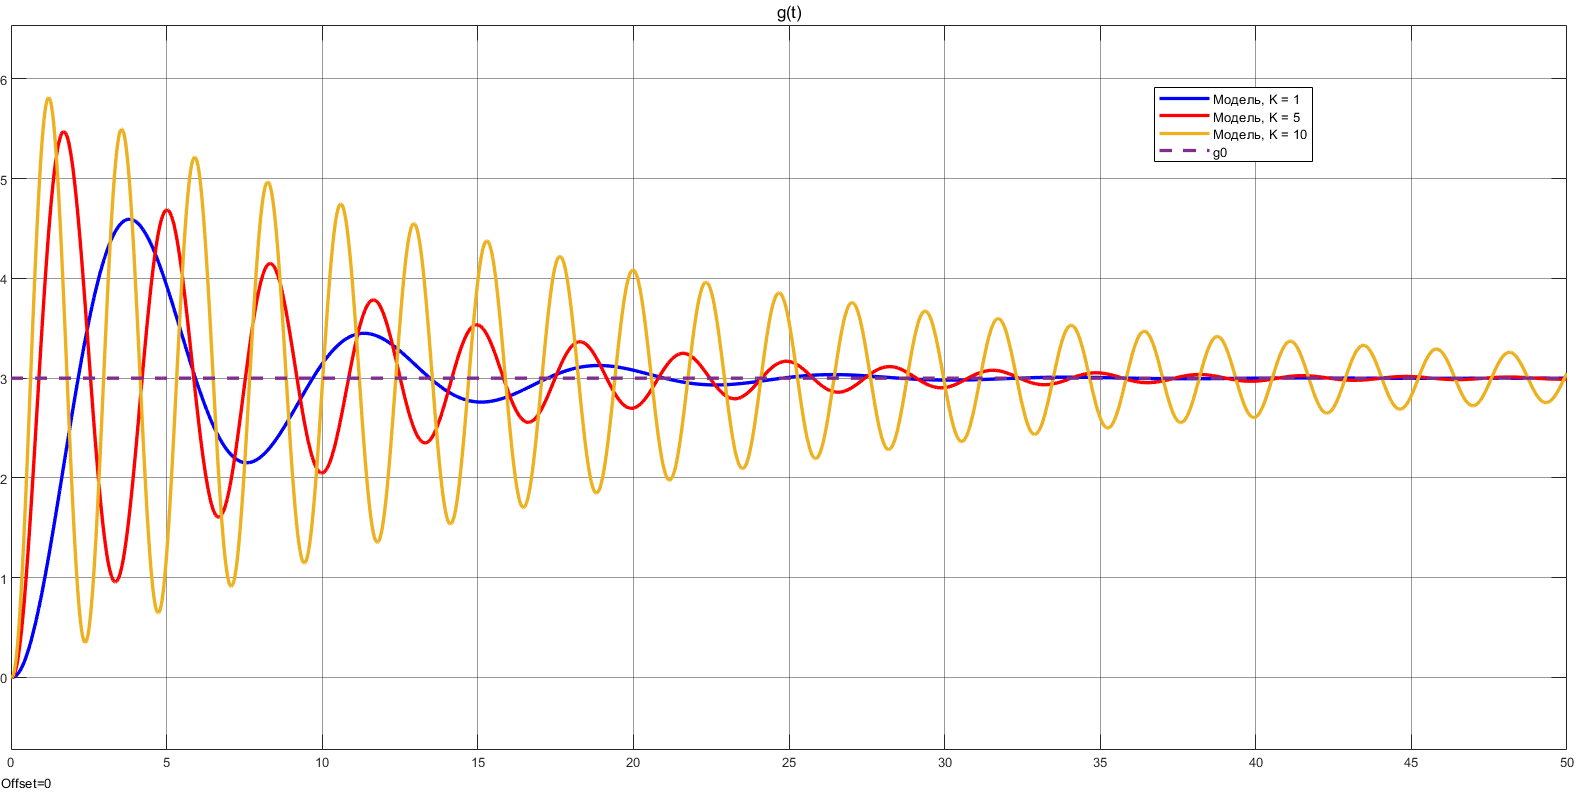
\includegraphics[width=\textwidth]{images/t2g1.png}
    \caption{Сравнительные графики $y(t)$ для задания 2, стационарного режима}
    \label{fig:2}
\end{figure}
Затем построим графики $e(t)$, для наглядности изобразим в тех же осях установившуюся ошибку $\varepsilon$:
\begin{figure}[H]
    \centering
    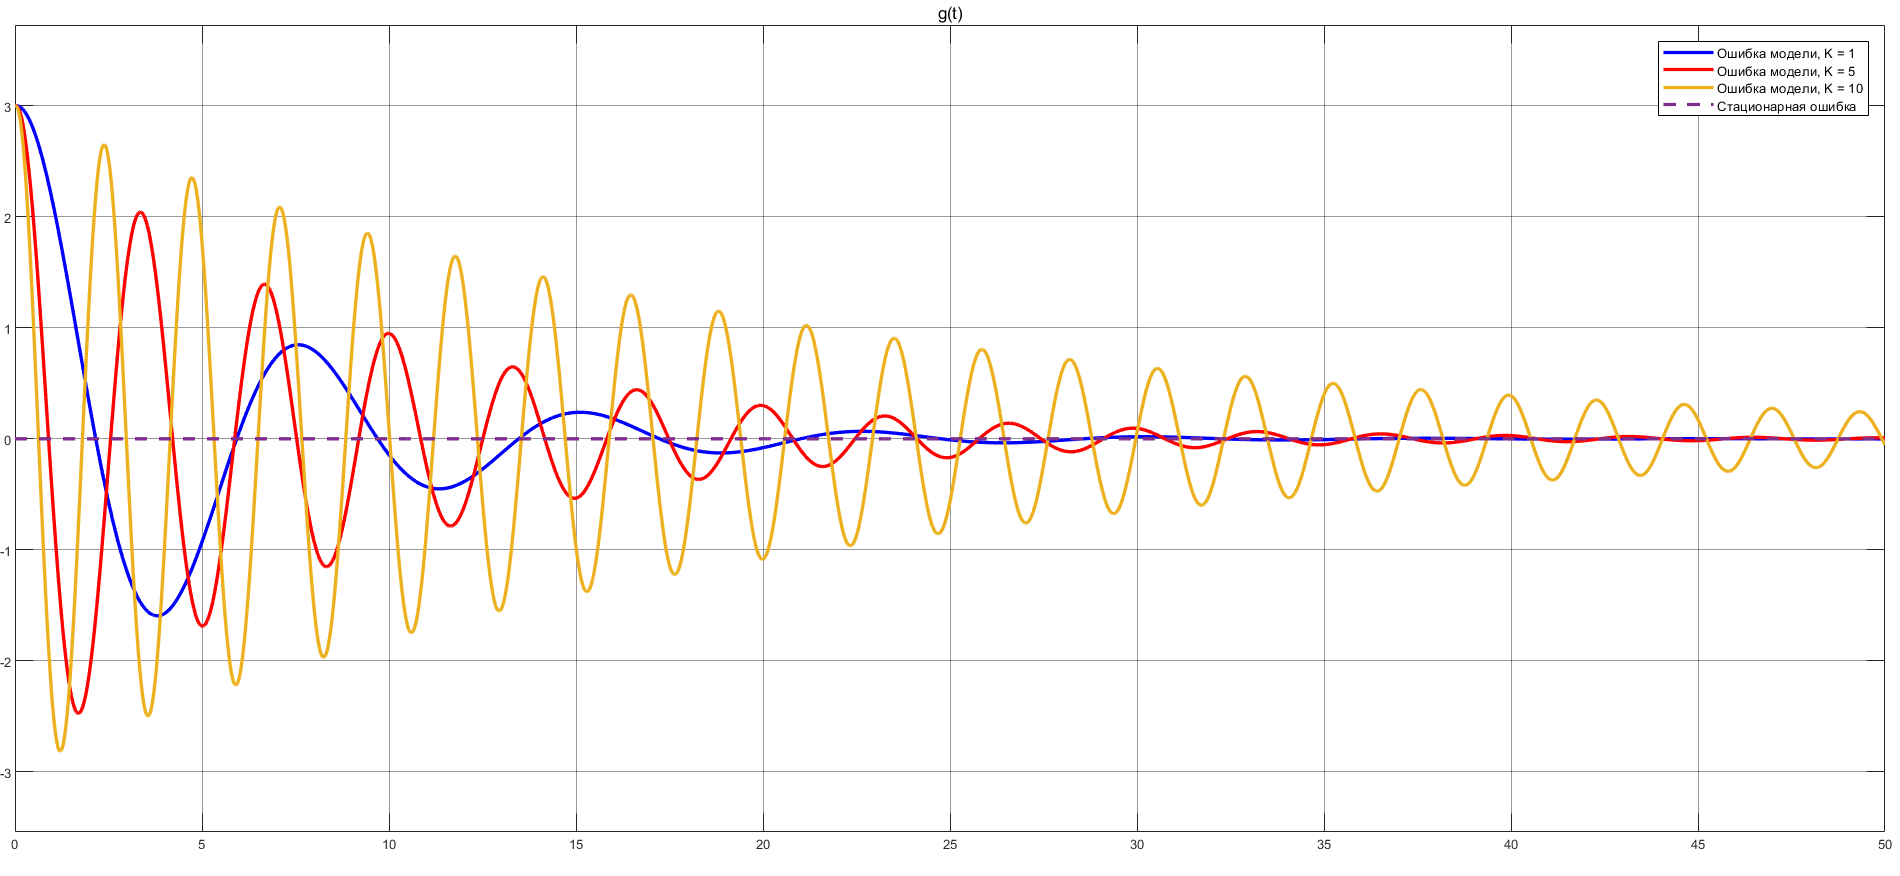
\includegraphics[width=\textwidth]{images/t2g2.png}
    \caption{Сравнительные графики $e(t)$ для задания 2, стационарного режима}
    \label{fig:2}
\end{figure}
\newpage
\subsection{Сравнительные графики для движения с постоянной скоростью}
\begin{figure}[H]
    \centering
    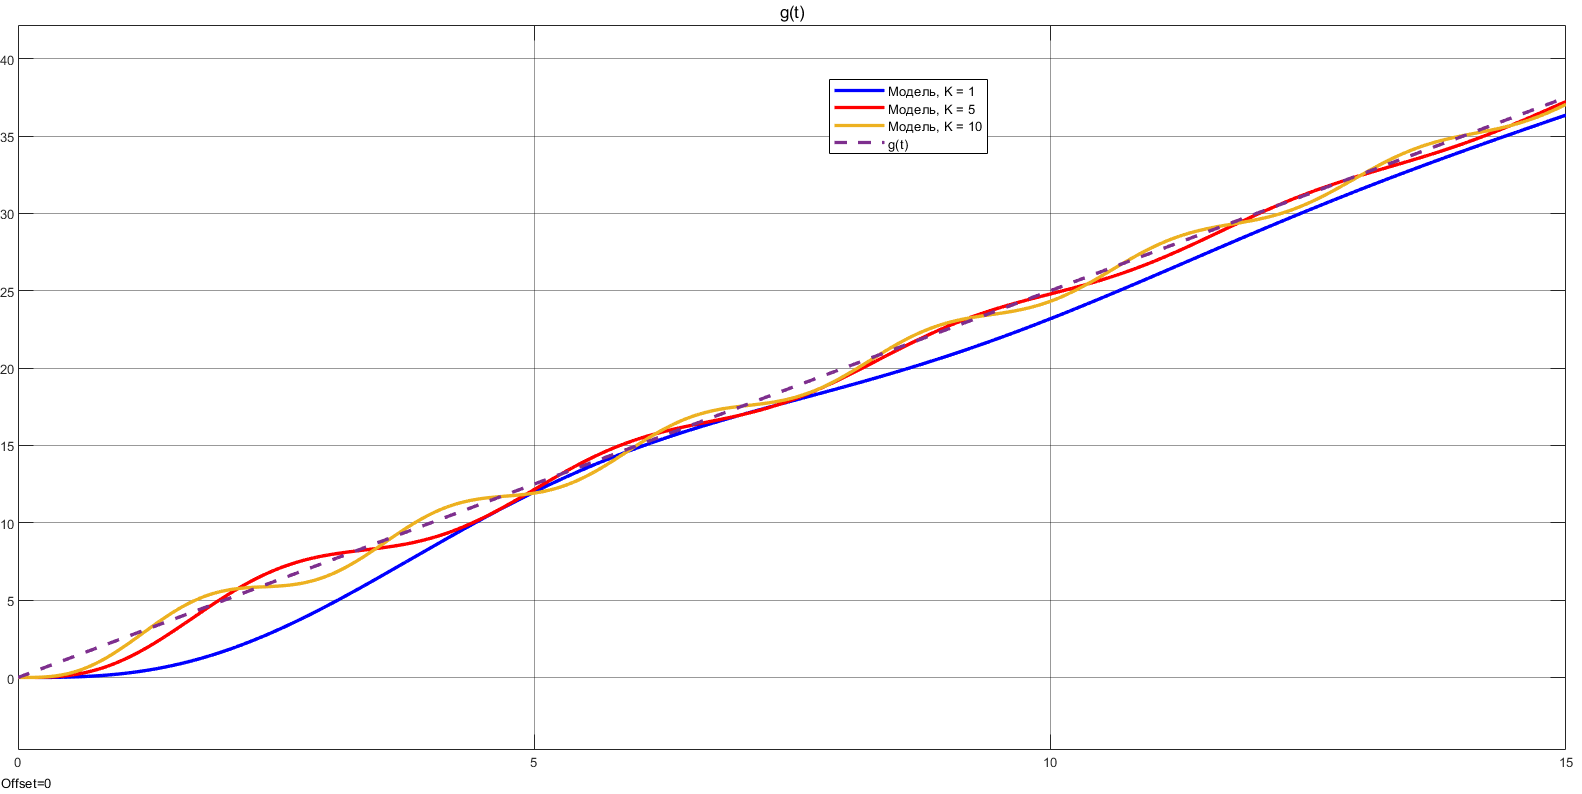
\includegraphics[width=\textwidth]{images/t2g3.png}
    \caption{Сравнительные графики $y(t)$ для задания 2, постоянной скорости}
    \label{fig:2}
\end{figure}
\begin{figure}[H]
    \centering
    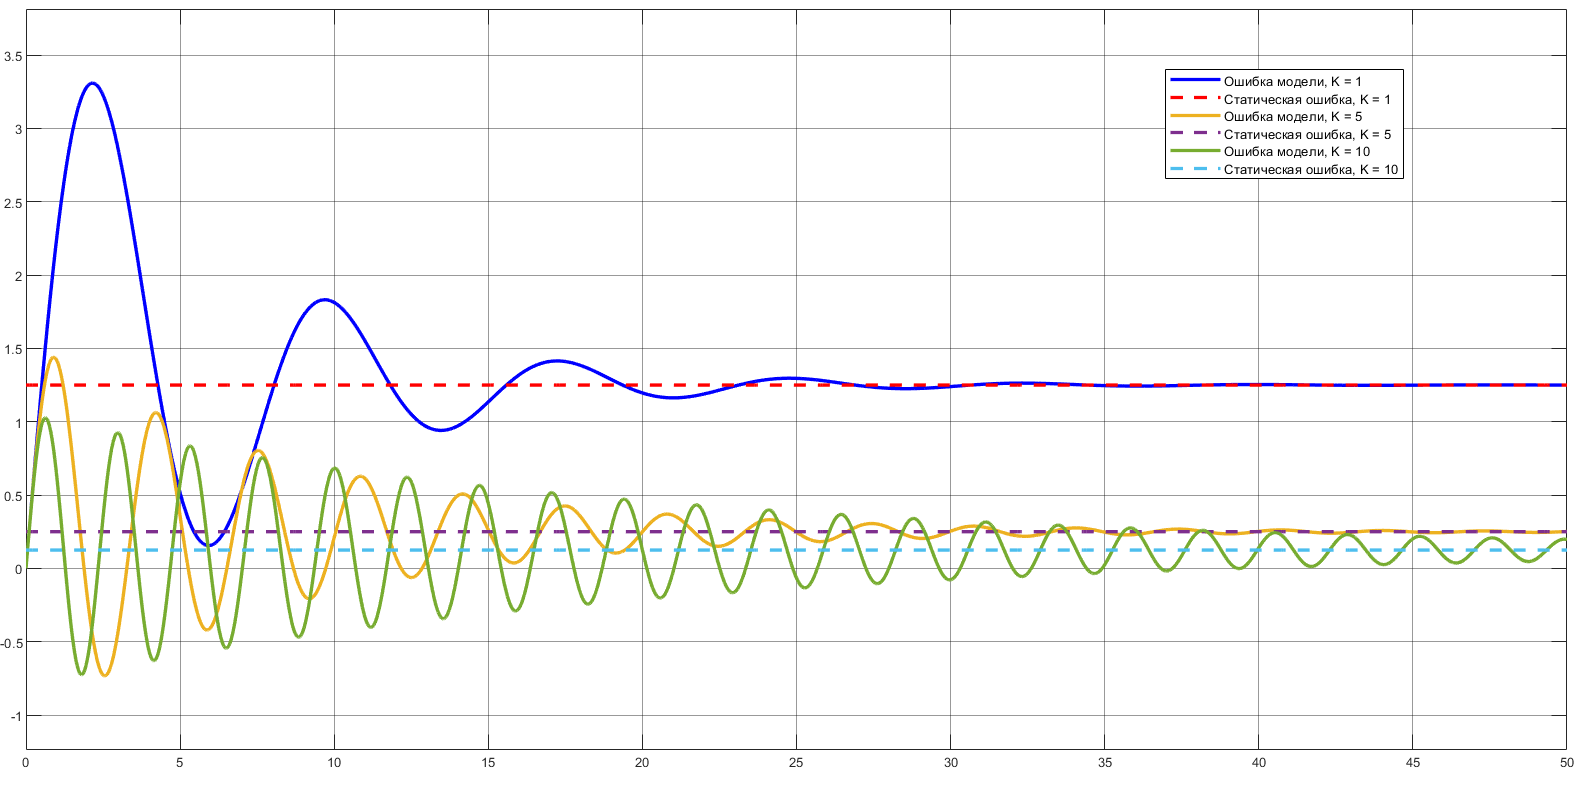
\includegraphics[width=\textwidth]{images/t2g4.png}
    \caption{Сравнительные графики $e(t)$ для задания 2, постоянной скорости}
    \label{fig:2}
\end{figure}
\newpage
\subsection{Сравнительные графики для движения с постоянным ускорением}
\begin{figure}[H]
    \centering
    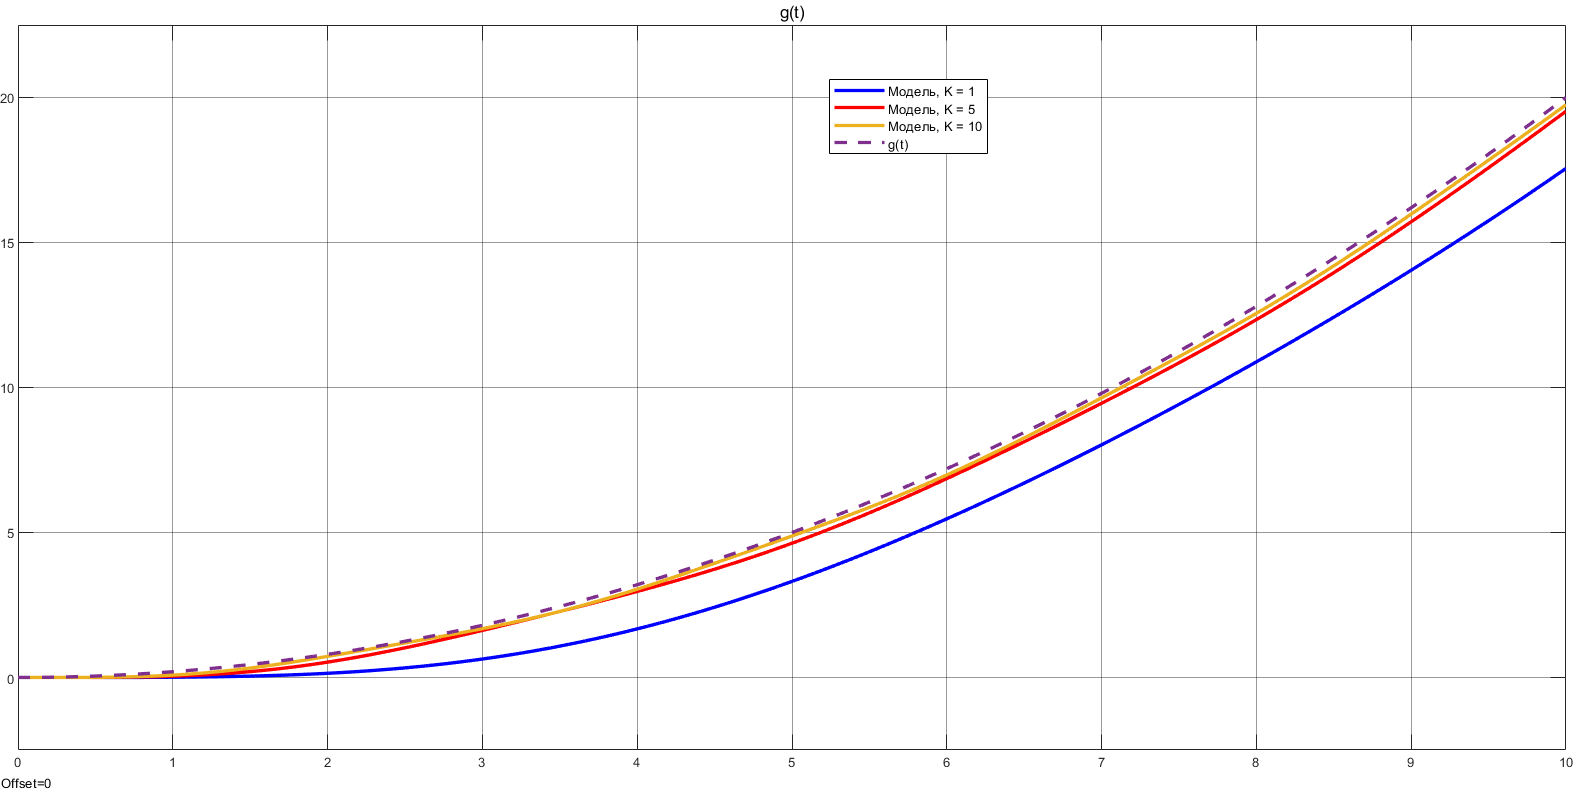
\includegraphics[width=\textwidth]{images/t2g5.png}
    \caption{Сравнительные графики $y(t)$ для задания 2, постоянного ускорения}
    \label{fig:2}
\end{figure}
\begin{figure}[H]
    \centering
    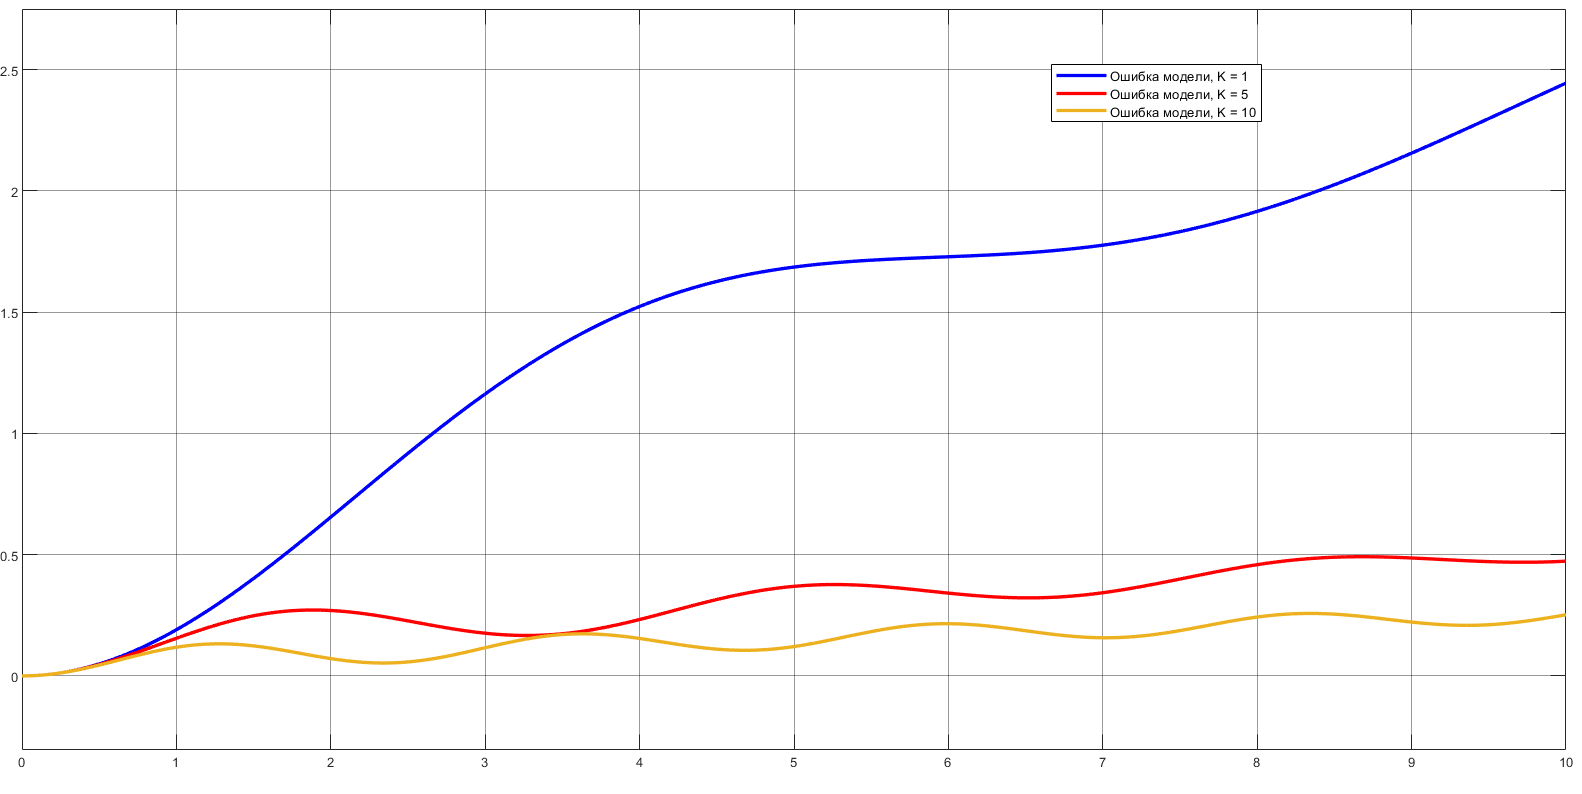
\includegraphics[width=\textwidth]{images/t2g6.png}
    \caption{Сравнительные графики $e(t)$ для задания 2, постоянного ускорения}
    \label{fig:2}
\end{figure}
\newpage
\subsection{Выводы по заданию 2}
В результате моделирования линейной системы с интегральным регулятором в стационарном режиме и в режиме с постоянной скоростью было получено соответствие вычисленной теоретически статической ошибки и результатов моделирования. Также из результатов моделирования можно сделать вывод что при увеличении коэффициента интегрального регулятора уменьшается установившаяся ошибка в режиме с постоянной скоростью и увеличивается время переходного процесса.
\newline
При моделировании же этой системы в режиме движения с постоянным ускорением было получено, что ошибка неограничено возрастает с течением времени (что соответствует первому порядку астатизма системы). При этом увеличение коэффициента интегрального регулятора снижает скорость роста ошибки.
\newpage
\section{ПИ-регулятор}
\subsection{Схема моделирования системы}
Совместим пропорциональный и интегральный регулятор, сложив их передаточные функции и получим пропорционально-интегральный (ПИ) регулятор. Построим схему моделирования с ПИ-регулятором:
\begin{figure}[H]
    \centering
    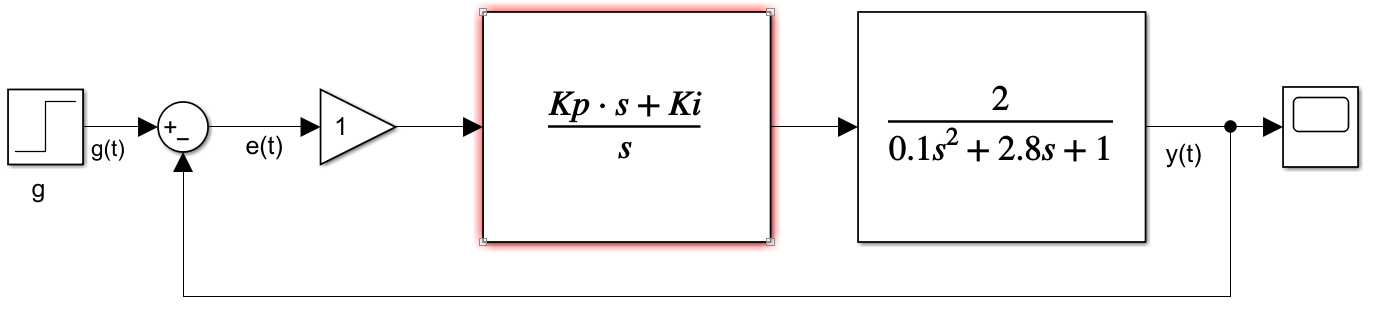
\includegraphics[width=\textwidth]{images/model3.png}
    \caption{Схема моделирования задания 3}
    \label{fig:1}
\end{figure}
\subsection{Аналитический расчет предельного значения установившейся ошибки}
Проверим ассимптотическую устойчивость системы. Для этого найдем полную передаточную функцию системы по ошибке как:
\[
    W(s)_{g \rightarrow e} = \frac{1}{1 + H(s)W_{\textit{упр}}(s)} = \frac{1}{\frac{0,1s^3 + 2,8s^2 + (1 + 2K_p)s + 2K_i}{0,1s^3 + 2,8s^2 + s}} = \frac{0,1s^3 + 2,8s^2 + s}{0,1s^3 + 2,8s^2 + (1 + 2K_p)s + 2K_i}
\]
Составим матрицу Гурвица:
\[
    H = \begin{pmatrix}
    2,8 & 2K_i & 0 \\
    0.1 & 1+2K_p & 0 \\
    0 & 2,8 & 2K_i
\end{pmatrix}
\]
Найдем определители ее угловых матриц:
\[
    \Delta_1 = 2,8
\]
\[
    \Delta_2 = 2,8 + 5,6K_p - 0.2K_i
\]
\[
    \Delta_3 = 5,6K_i + 11,2K_p K_i - 0,4K_i^2 = 2K_i \Delta_2
\]
При $K_i, K_p \in \{1, 5, 10\}$ определители положительны, следовательно, система ассимптотически устойчива.
\newline
Найдем статическую ошибку в режиме движения с постоянной скоростью:
\[
    \varepsilon = \frac{V}{K_1} = \frac{2,5}{2K_i}
\]
Теперь можем построить для системы с ПИ-регулятором графики $y(t)$ и $e(t)$ при постоянной скорости c разными значениями $K_i$ и $K_p$:
\newpage
\subsection{Сравнительные графики для движения с постоянной скоростью}
\begin{figure}[H]
    \centering
    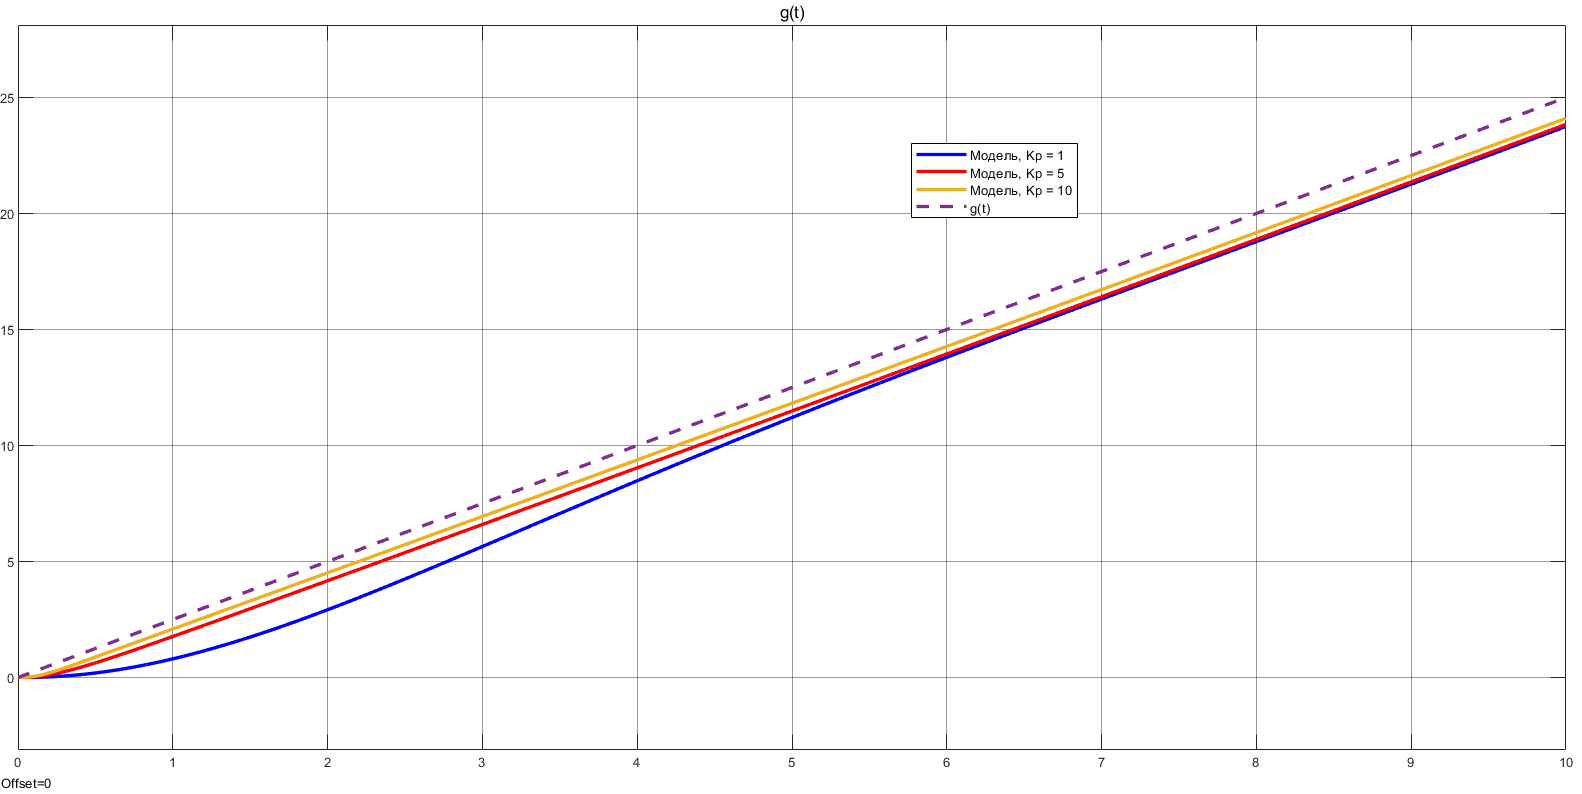
\includegraphics[width=\textwidth]{images/t3g1Ki1.png}
    \caption{Сравнительные графики $y(t)$ для задания 3, $K_i = 1$}
    \label{fig:2}
\end{figure}
\begin{figure}[H]
    \centering
    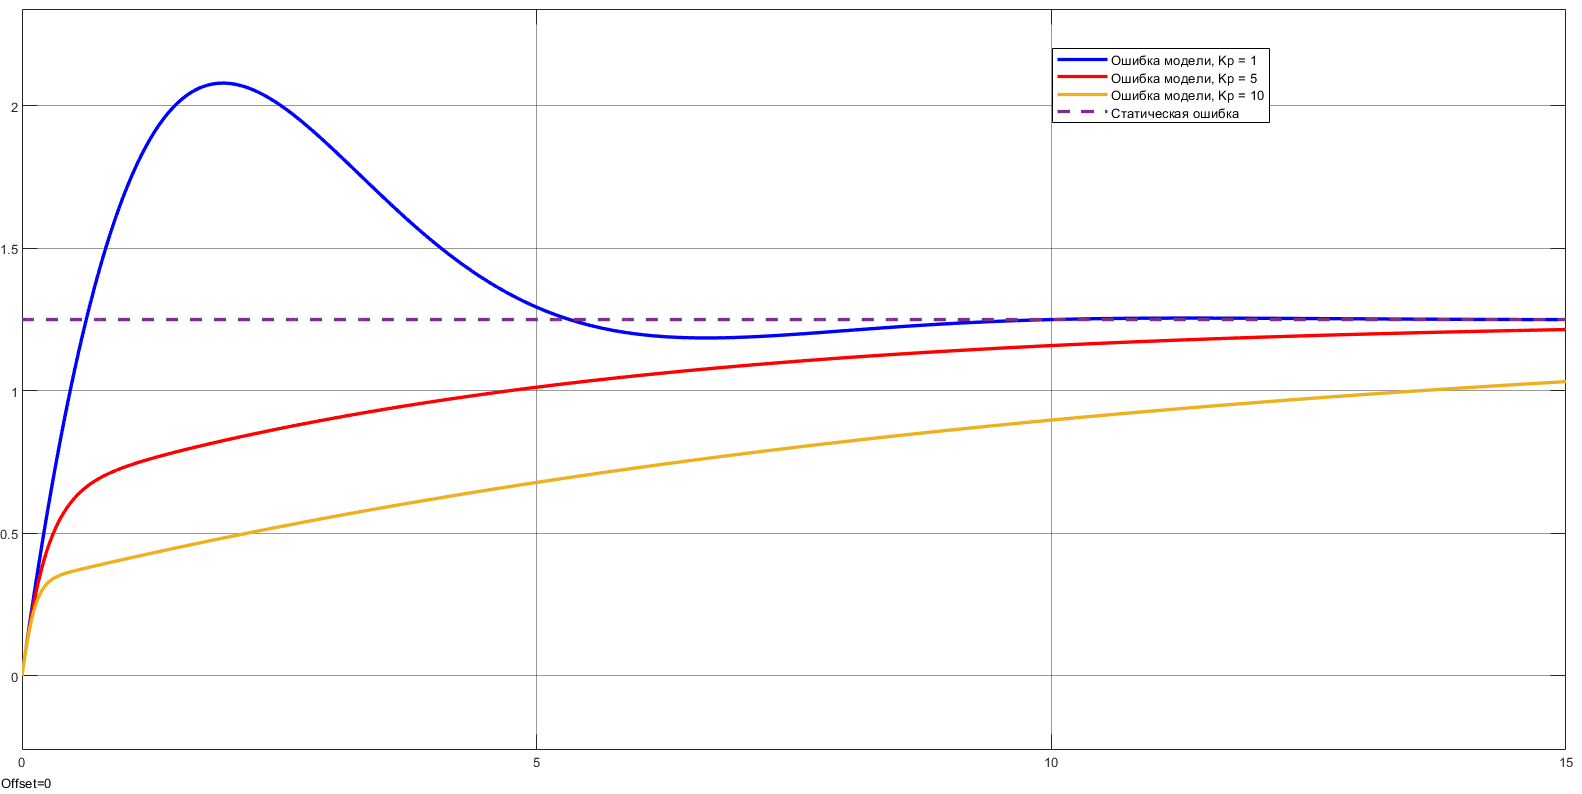
\includegraphics[width=\textwidth]{images/t3g2Ki1.png}
    \caption{Сравнительные графики $e(t)$ для задания 3, $K_i = 1$}
    \label{fig:2}
\end{figure}
\newpage
\begin{figure}[H]
    \centering
    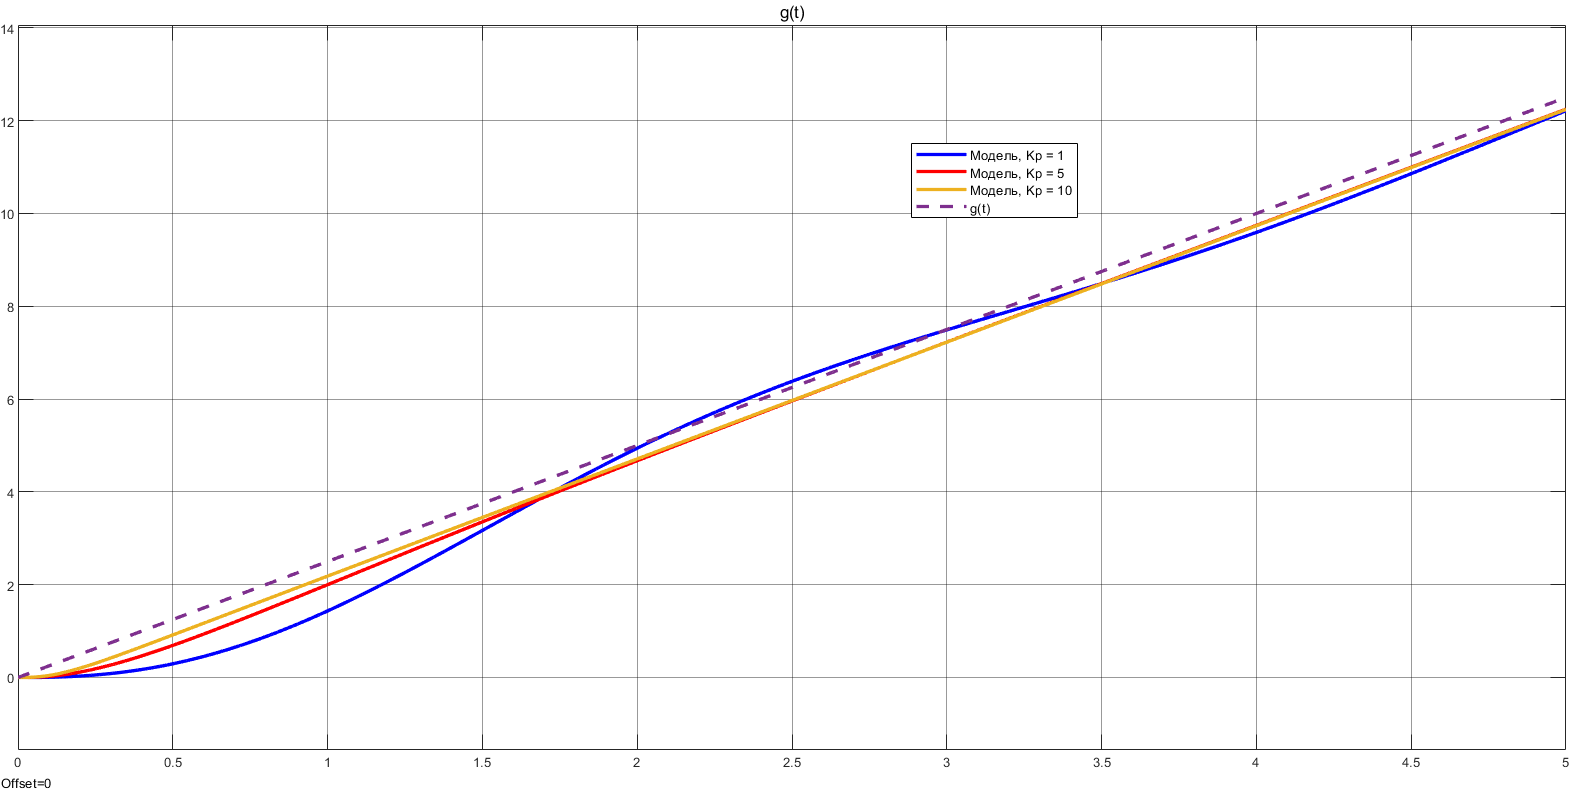
\includegraphics[width=\textwidth]{images/t3g1Ki5.png}
    \caption{Сравнительные графики $y(t)$ для задания 3, $K_i = 5$}
    \label{fig:2}
\end{figure}
\begin{figure}[H]
    \centering
    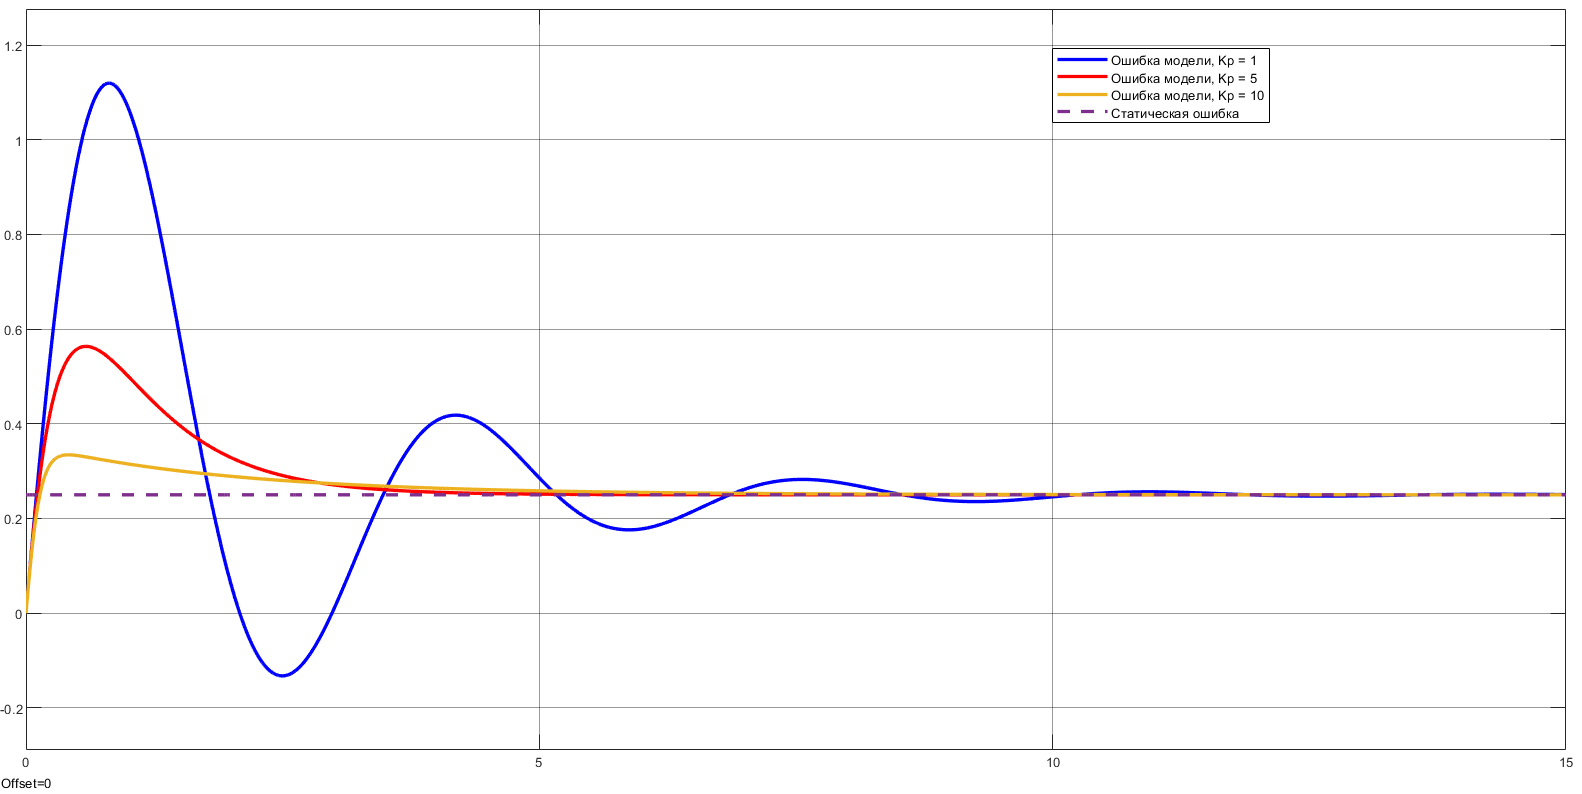
\includegraphics[width=\textwidth]{images/t3g2Ki5.png}
    \caption{Сравнительные графики $e(t)$ для задания 3, $K_i = 5$}
    \label{fig:2}
\end{figure}
\newpage
\begin{figure}[H]
    \centering
    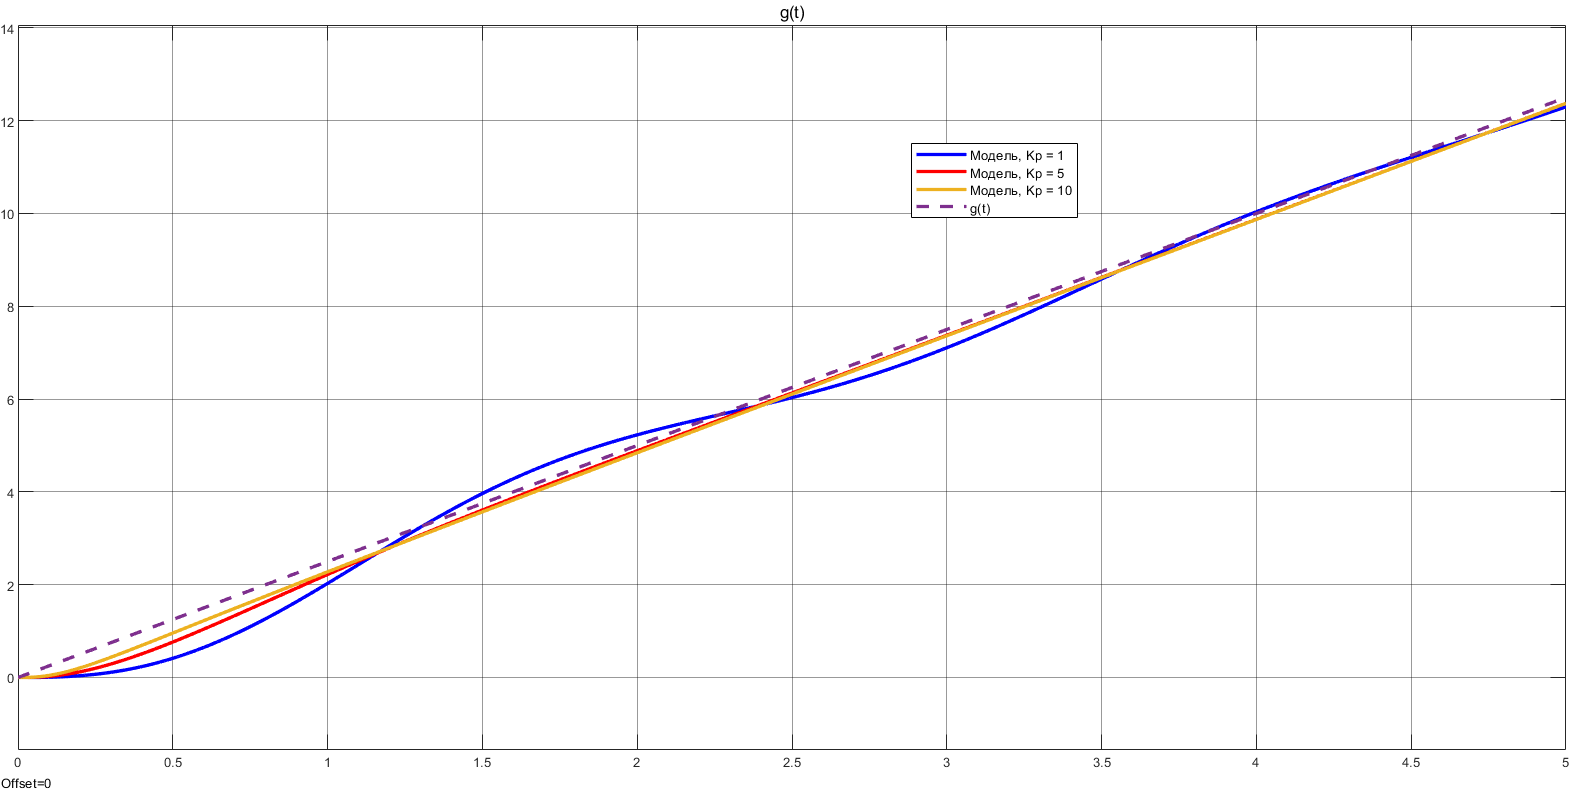
\includegraphics[width=\textwidth]{images/t3g1Ki10.png}
    \caption{Сравнительные графики $y(t)$ для задания 3, $K_i = 10$}
    \label{fig:2}
\end{figure}
\begin{figure}[H]
    \centering
    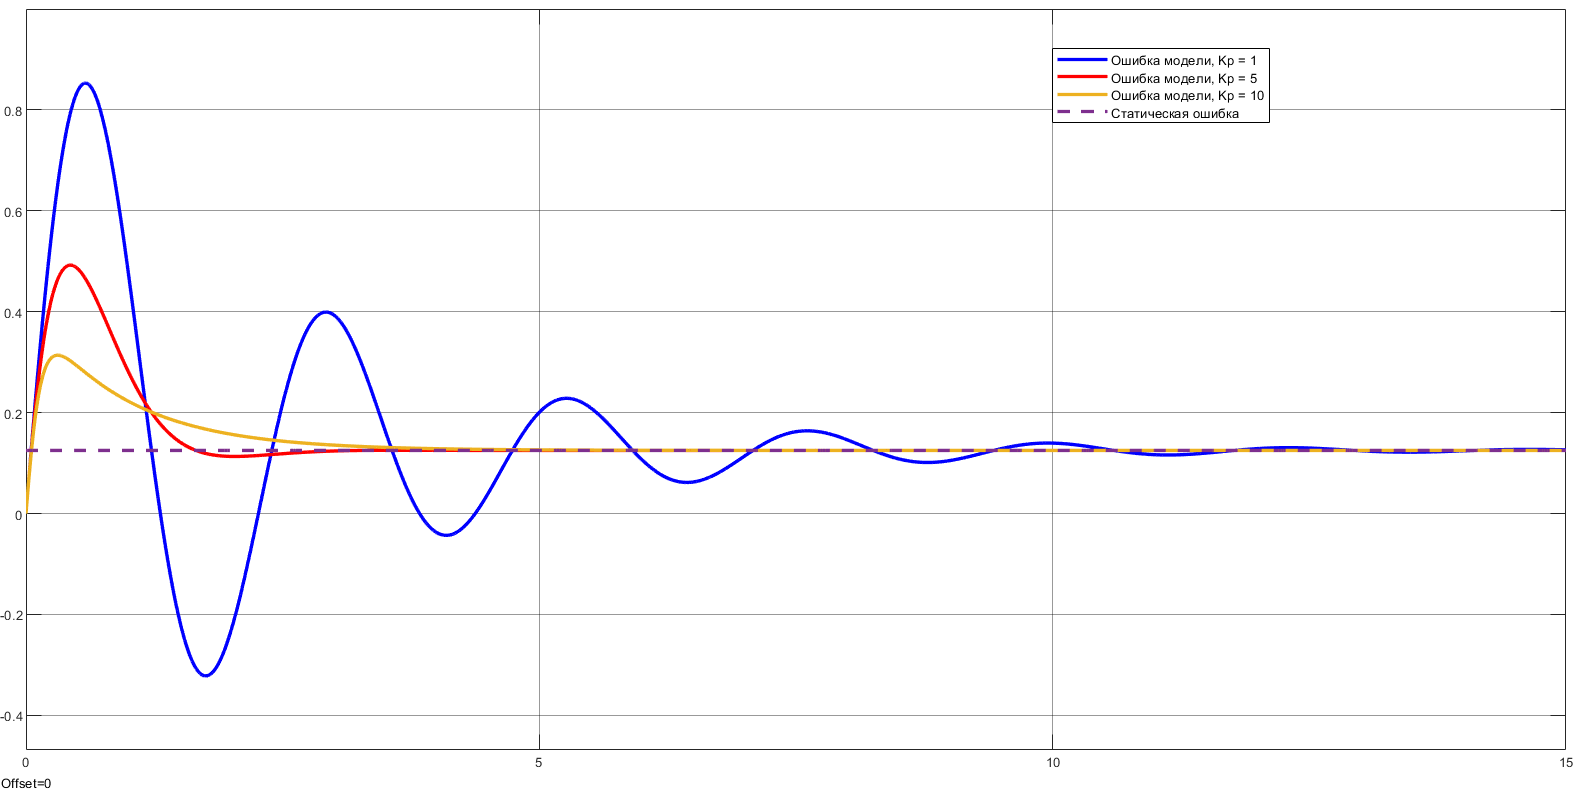
\includegraphics[width=\textwidth]{images/t3g2Ki10.png}
    \caption{Сравнительные графики $e(t)$ для задания 3, $K_i = 10$}
    \label{fig:2}
\end{figure}
\newpage
\subsection{Выводы по заданию 3}
Видим, что при использовании ПИ-регулятора в режиме постоянной скорости результаты моделирования совпадают с найденной теоретически статической ошибкой. При этом, при увеличении $K_i$ уменьшается установившаяся ошибка, но при малом $K_p$ увеличивается время переходного процесса. Однако, при большом $K_p$ увеличение $K_i$ может даже уменьшить время переходного процесса.
\newpage
\section{Задание 4. Внешние возмущения}
\subsection{Схема моделирования системы}
Составим схему системы с фиксированными внешними возмущениями:
\begin{figure}[H]
    \centering
    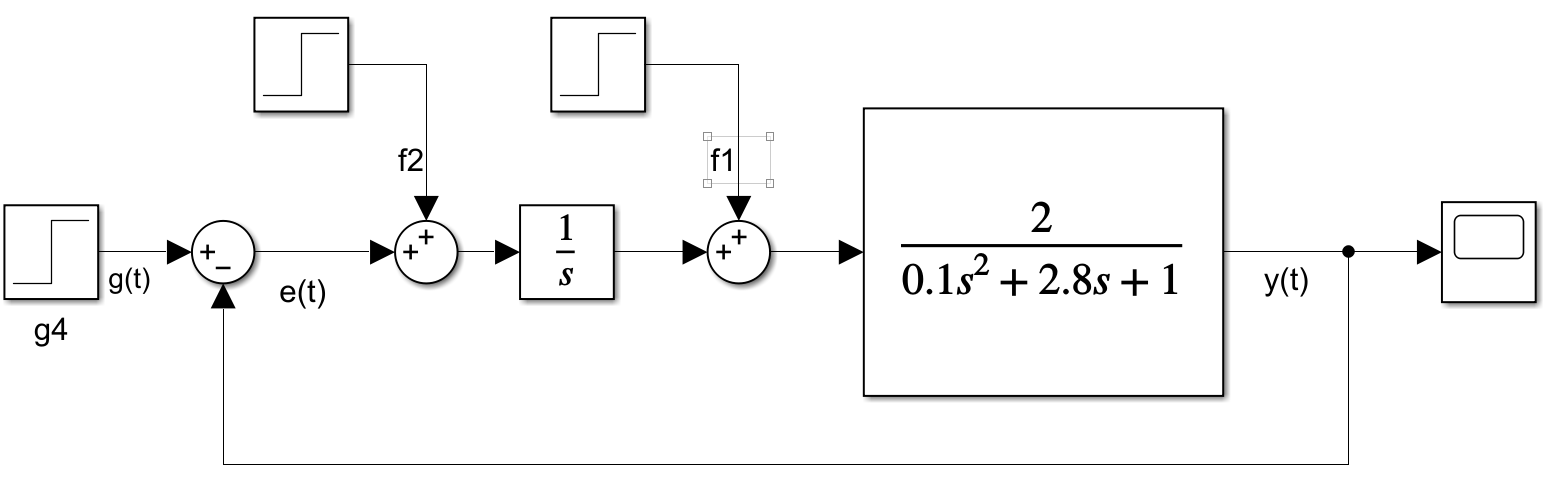
\includegraphics[width=\textwidth]{images/model4.png}
    \caption{Схема моделирования задания 4}
    \label{fig:1}
\end{figure}
Переместим прибавление $g$ через сложение, получим эквивалентную схему и избавимся от входного сигнала:
\begin{figure}[H]
    \centering
    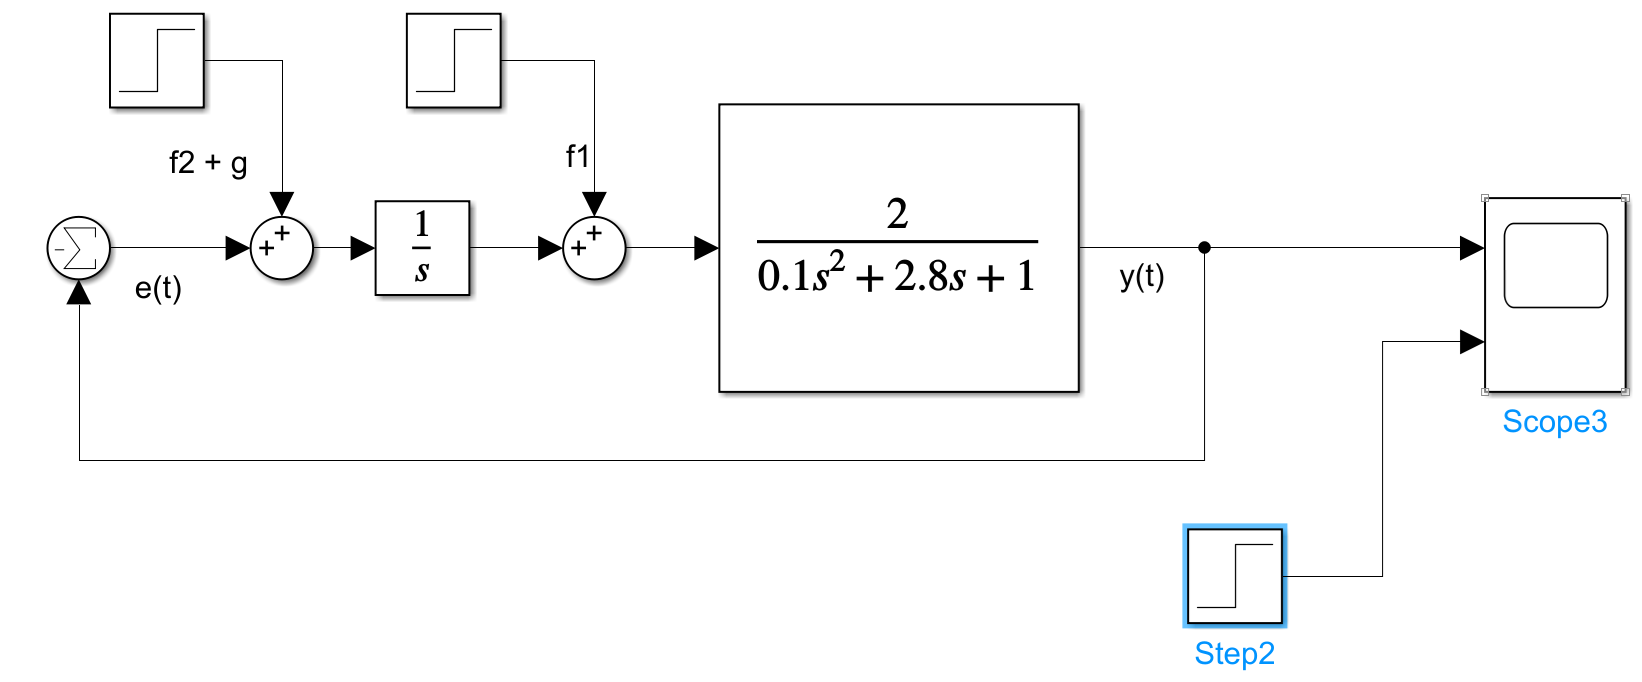
\includegraphics[width=\textwidth]{images/model41.png}
    \caption{Схема моделирования задания 4 после преобразования}
    \label{fig:1}
\end{figure}
\subsection{Расчет статической ошибки при нуле одного из возмущений и стационарном воздействии}
Примем $g(t) = 1(t)$, $f_2(t) = 0$, $f_1(t) = F_1(t)$:
\newline
Запишем выражение для ошибки:
\[
    e(t) = -y(t) = -\frac{1}{s}W(s)[1(t)] - W(s)[F_1(t) + \frac{1}{s}[e(t)]] 
\]
\[
    e(t) = -\frac{1}{s}W(s)[1(t)] - W(s)[F_1(t)] - \frac{1}{s}W(s)[e(t)]
\]
\[
    (1 + \frac{1}{s}W(s))[e] = -\frac{1}{s}W(s)[1(t)] - W(s)[F_1(t)]
\]
\[
    e = -\frac{\frac{1}{s}W(s)}{1 + \frac{1}{s}W(s)}[1(t)] - \frac{W(s)}{1 + \frac{1}{s}W(s)}[F_1(t)] = -\frac{W(s)}{s + W(s)}[1(t)] - \frac{sW(s)}{s + W(s)}[F_1(t)] = \frac{W(s) - F_1sW(s)}{s + W(s)}[1(t)]
\]
Тогда, статическую ошибку можно представить как:
\[
    \varepsilon_1 = \lim_{s \to 0}(s\frac{-W(s) - F_1sW(s)}{s + W(s)}\frac{1}{s}) = \lim_{s \to 0}(\frac{\frac{2}{0,1s^2 + 2,8s + 1} - F_1\frac{2s}{0,1s^2 + 2,8s + 1}}{s + \frac{2}{0,1s^2 + 2,8s + 1}}) =
\]
\[
    = \lim_{s \to 0}(\frac{2 - 2sF_1}{0,1s^2 + 2,8s + 1} / \frac{0,1s^3 + 2,8s^2 + s + 2}{0,1s^2 + 2,8s + 1}) = \lim_{s \to 0}(\frac{2 - 2sF_1}{0,1s^3 + 2,8s^2 + s + 2}) = 1
\]
\newline
Теперь примем $g(t) = 1(t)$, $f_2(t) = F_2$, $f_1(t) = 0$:
\newline
Запишем выражение для ошибки:
\[
    e(t) = - y = -\frac{1}{s}W(s)[1(t)] - W(s)[\frac{1}{s}[e(t) + F_2(t)]] 
\]
\[
    e(t) = -\frac{1}{s}W(s)[1(t)] - \frac{1}{s}W(s)[F_2(t)] - \frac{1}{s}W(s)[e(t)]
\]
\[
    (1 + \frac{1}{s}W(s))[e] = -\frac{1}{s}W(s)[1(t)] - \frac{1}{s}W(s)[F_2(t)]
\]
\[
    e = -\frac{\frac{1}{s}W(s)}{1 + \frac{1}{s}W(s)}[1(t)] - \frac{\frac{1}{s}W(s)}{1 + \frac{1}{s}W(s)}[F_2(t)] = \frac{W(s)}{s + W(s)}[1(t)] - \frac{W(s)}{s + W(s)}[F_2(t)] = \frac{W(s) - F_2W(s)}{s + W(s)}[1(t)]
\]
Тогда, статическую ошибку можно представить как:
\[
    \varepsilon_2 = \lim_{s \to 0}(s\frac{-W(s) - F_2W(s)}{s + W(s)}\frac{1}{s}) = \lim_{s \to 0}(\frac{-\frac{2}{0,1s^2 + 2,8s + 1} - F_2\frac{2}{0,1s^2 + 2,8s + 1}}{s + \frac{2}{0,1s^2 + 2,8s + 1}}) =
\]
\[
    = \lim_{s \to 0}(\frac{0,1s^3 + 2,8s^2 + s - 2F_2}{0,1s^2 + 2,8s + 1} / \frac{0,1s^3 + 2,8s^2 + s + 2}{0,1s^2 + 2,8s + 1}) = \lim_{s \to 0}(\frac{0,1s^3 + 2,8s^2 + s - 2F_2}{0,1s^3 + 2,8s^2 + s + 2}) = -(1 + F_2)
\]
\newpage
\subsection{Графики $e(t)$ для системы с возмущениями при нуле одного из возмущений}
\begin{figure}[H]
    \centering
    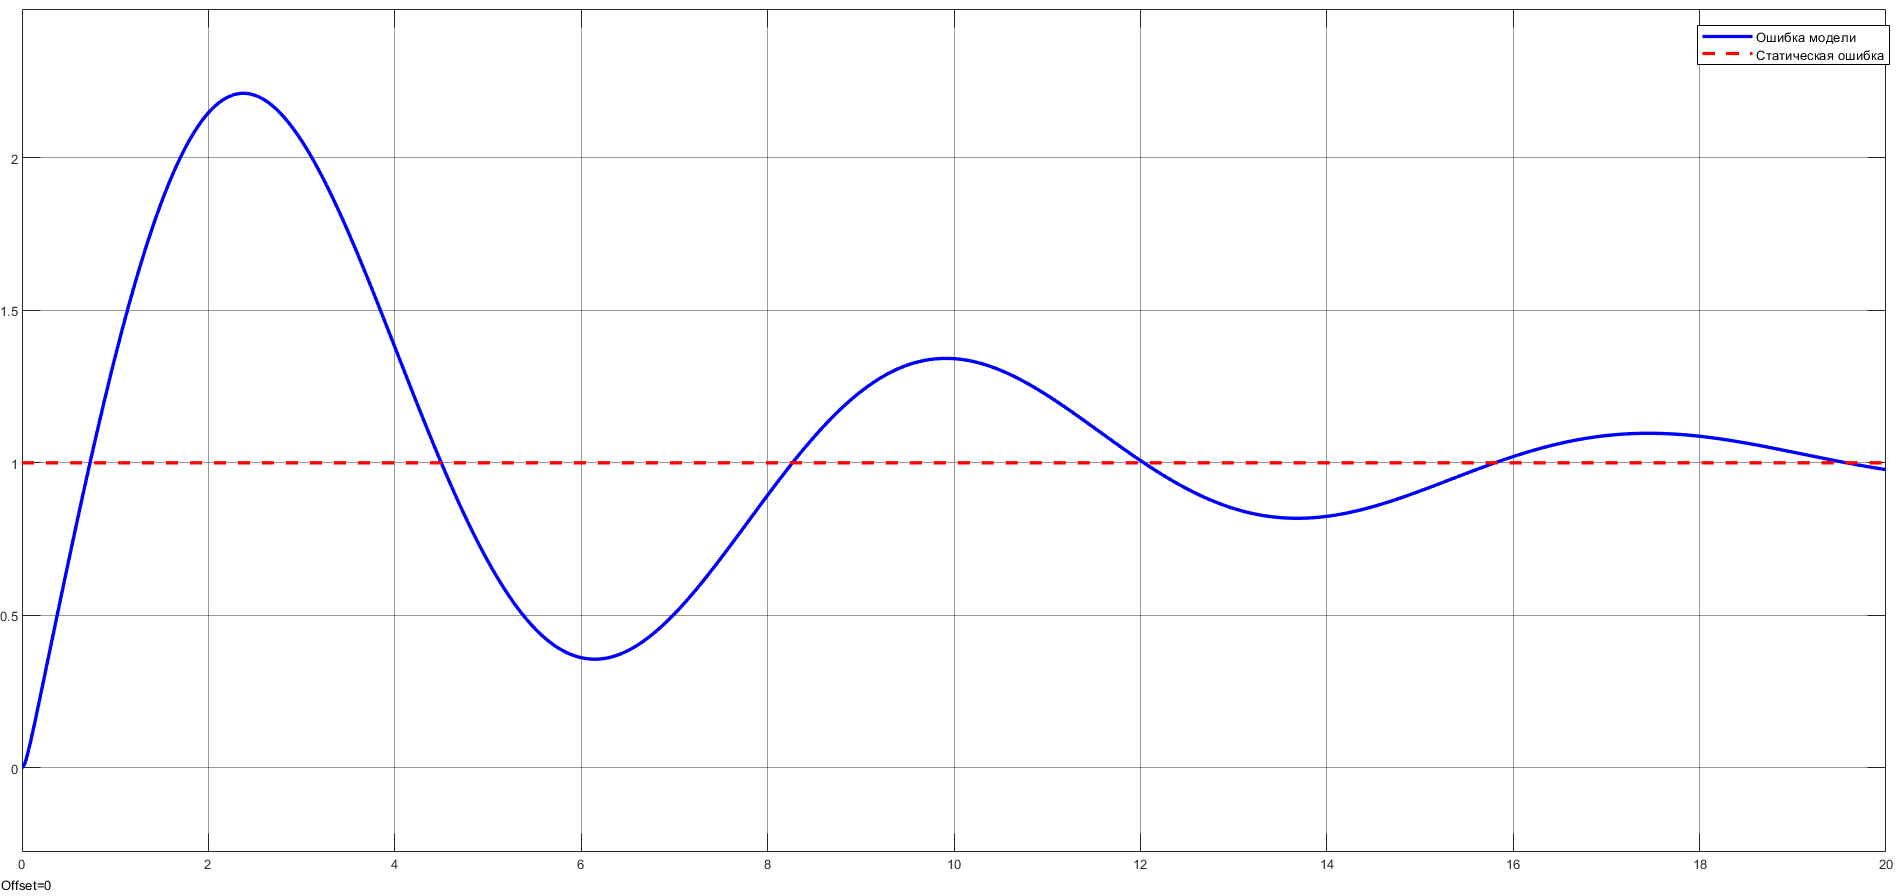
\includegraphics[width=\textwidth]{images/t4g1.png}
    \caption{Сравнительные графики $e(t)$ для задания 4, ненулевое первое возмущение}
    \label{fig:2}
\end{figure}
\begin{figure}[H]
    \centering
    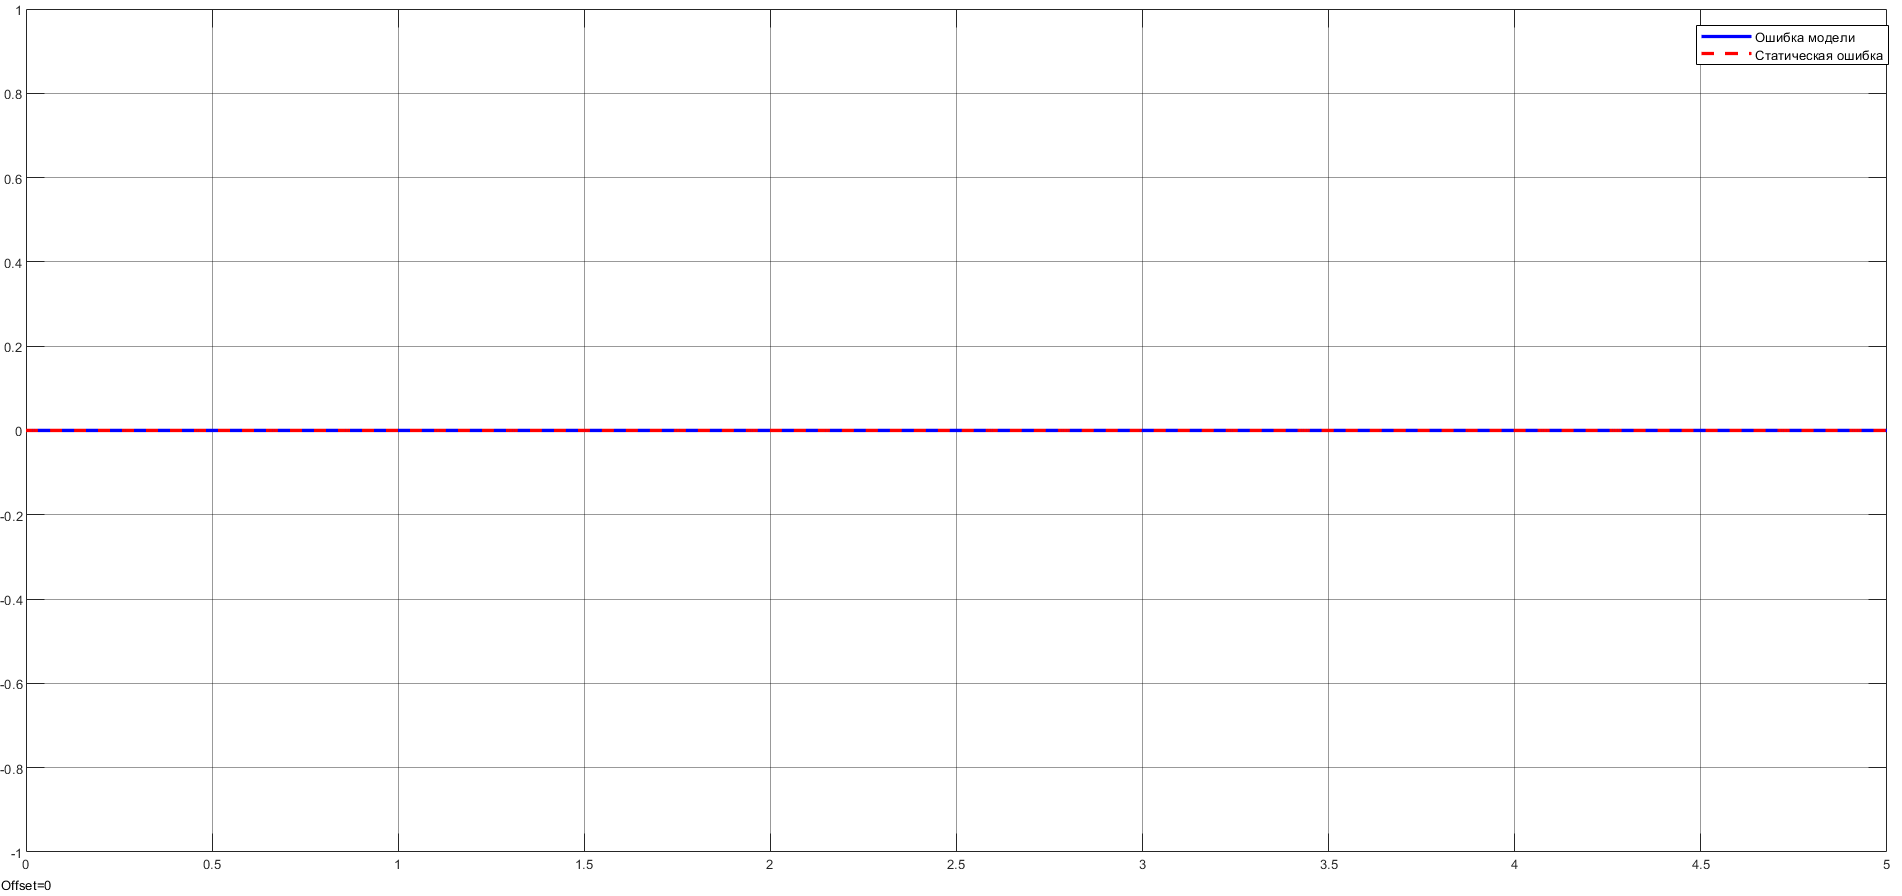
\includegraphics[width=\textwidth]{images/t4g2.png}
    \caption{Сравнительные графики $e(t)$ для задания 4, ненулевое второе возмущение}
    \label{fig:2}
\end{figure}
\newpage
\subsection{Выводы по 4 заданию}
Видим, что вычисленная теоретически установившаяся ошибка совпала с моделированием.
\newpage
\section{Задание 5}
\subsection{Схема моделирования системы}
Построим схему моделирования системы с линейным входом ($4 + 4t$) без регулятора:
\begin{figure}[H]
    \centering
    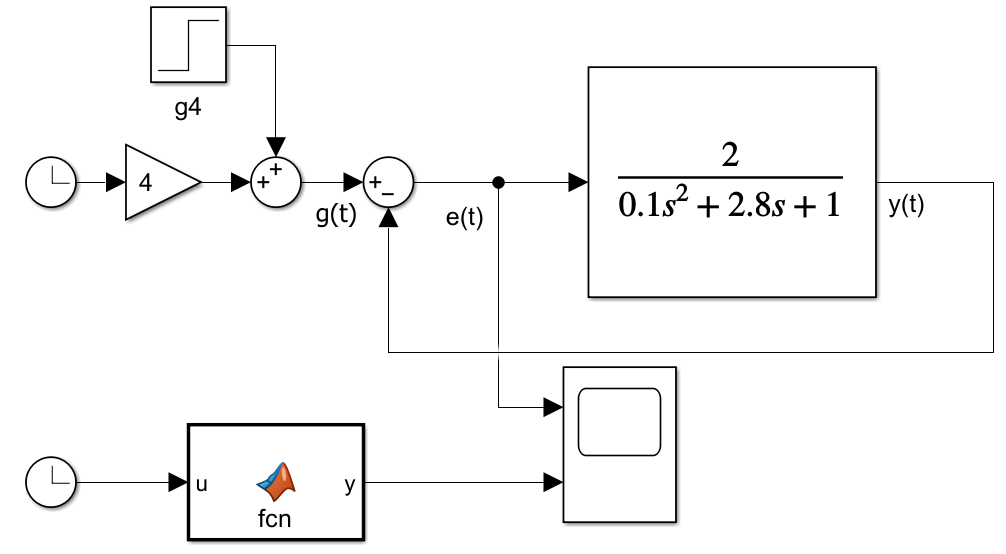
\includegraphics[width=\textwidth]{images/model5.png}
    \caption{Схема моделирования задания 5}
    \label{fig:1}
\end{figure}
\subsection{Приближенный расчет установившейся ошибки с помощью ряда Тейлора}
\[
    e_y(t) = \sum_{i=0}^{\infty}\frac{c_i \cdot g(t)^{(i)}}{i!}
\]
При этом:
\[
    c_i = W_{g \to e}(s)^{(n)}, \ \ \textit{при} \ \ s \to 0
\]
Найдем передаточную функцию системы по ошибке $W_{g \to e}(s)$:
\[
    W_{g \to e}(s) = \frac{1}{1 + W(s)} = \frac{1}{1 + \frac{2}{0,1s^2 + 2,8s + 1}} = \frac{0,1s^2 + 2,8s + 1}{0,1^2 + 2,8s + 3}
\]
\[
    c_0 = \frac{1}{3}
\]
\[
    W_{g \to e}(s)' = \frac{40s + 560}{(s^2 + 28s + 30)^2}
\]
\[
    c_1 = \frac{560}{900}
\]
\[
    W_{g \to e}(s)'' = -\frac{120s^2 + 3360s + 30160}{(s^2 + 28s + 30)^3}
\]
\[
    c_2 = -\frac{30160}{30^3} \ \ - \ \ \textit{ограничена при} \ \ x \to 0
\]
Теперь найдем производные $g(t)$:
\[
    g(t) = 4t + 4
\]
\[
    g'(t) = 4
\]
\[
    g''(t) = 0
\]
Отсюда:
\[
    e_y(t) \approx \frac{1}{3} \cdot (4t + 4) + \frac{56}{90} \cdot 4 + c_2 \cdot \frac{0}{2} = \frac{1}{3} \cdot (4t + 4) + \frac{56}{90} \cdot 4
\]
Теперь можем построить график модели и сравнить его с полученным приближением.
\newpage
\subsection{Сравнительный график ошибки модели и полученного приближения}
\begin{figure}[H]
    \centering
    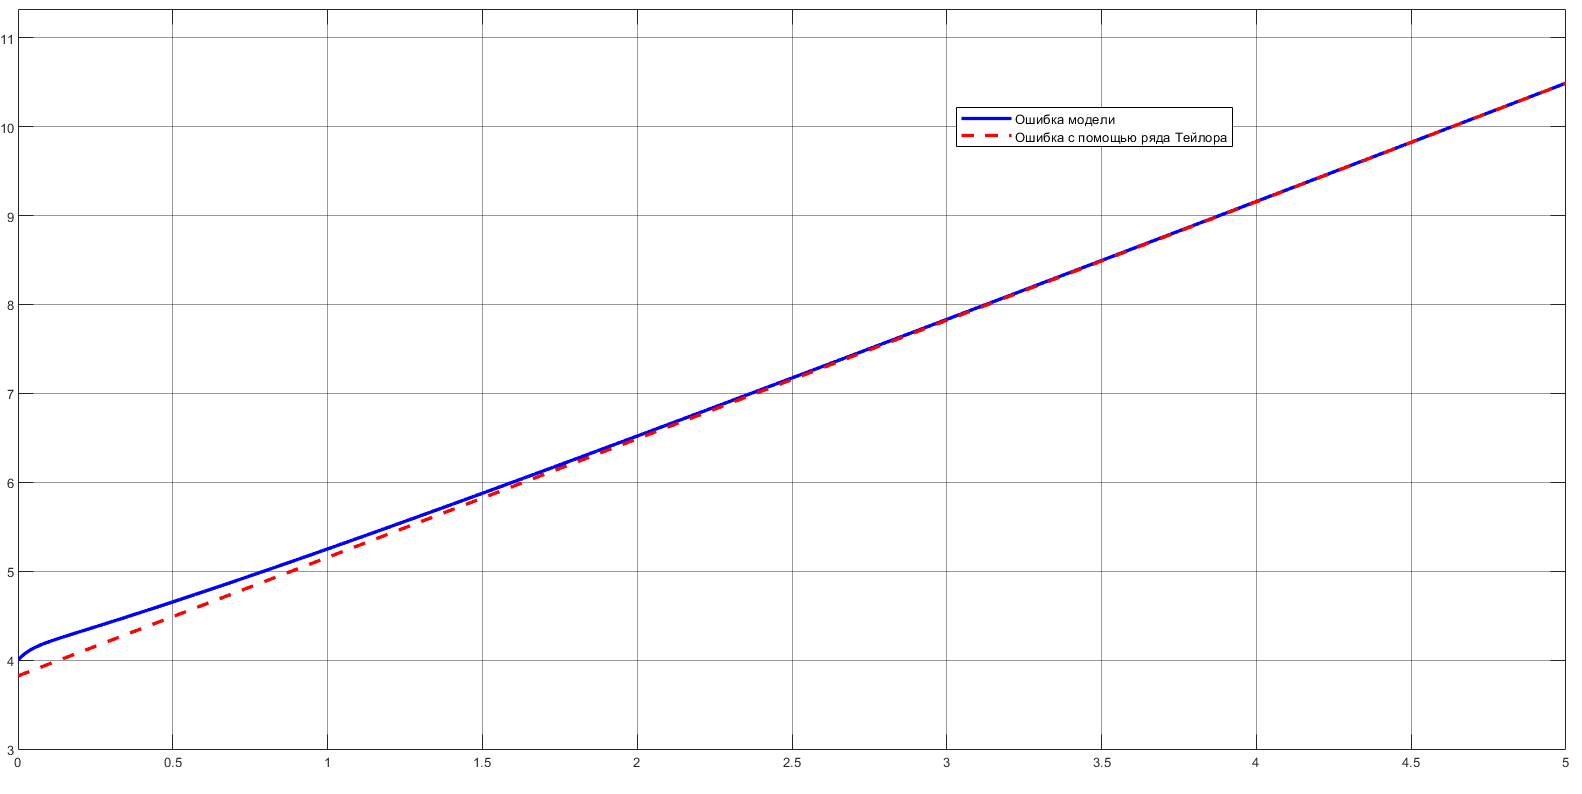
\includegraphics[width=\textwidth]{images/t5g1.png}
    \caption{Сравнительные графики $e(t)$ для задания 5}
    \label{fig:2}
\end{figure}
\newpage
\subsection{Выводы по 5 заданию}
Видим, что при возрастании $t$ приближение ошибки рядом Тейлора приближается к ошибке модели как и должно быть.
\section{Вывод}
В лабораторной работе была исследована линейная система управления с различными входными воздействиями и регуляторами. Для пропорционального, интегрального и пропорционально-интегрального регуляторов было проведено сравнение статической ошибки из теоретических соображений и из моделирования, результаты достаточно близко совпали.
\newline
Для этих регуляторов было проведено сравнение их работы при разных коэффициентах, сделаны выводы о поведении скорости переходного процесса и установившейся ошибки.
\newline
Также было проведено моделирование данной системы с постоянным возмущающим воздействием и с линейной функцией в качестве входного воздействия, установившаяся ошибка модели и из теоретических соображений в этих случах также совпали.
\end{document}


